\documentclass[12pt,a4paper,boxed,titlepage]{caspset}

% set 1-inch margins in the document
%\usepackage[left=1in,right=1in,top=1.2in,bottom=1in]{geometry}
\usepackage[left=1in,right=1in,top=1.2in,bottom=1in]{geometry}
\usepackage{lastpage}

% include this if you want to import graphics files with /includegraphics
\usepackage{multicol} 
\usepackage{capt-of}%%To get the caption
\usepackage{graphicx}
\usepackage{lscape}
\usepackage{amsmath,amsfonts,amsthm,amssymb}
\usepackage{mathtools}
\usepackage{hyperref}
\usepackage{setspace}
\usepackage{fancyhdr}
\usepackage{lastpage}
\usepackage{extramarks}
\usepackage{chngpage}
\usepackage{soul}
\usepackage[usenames,dvipsnames]{color}
\usepackage{graphicx,float,wrapfig}
\usepackage{ifthen}
\usepackage{listings}
\usepackage{courier}
\usepackage{multimedia}
\usepackage[toc,page,title,titletoc,header]{appendix}
\usepackage{color, soul}
\usepackage{tikz}
\usepackage{array}
\usepackage{multirow}
\usepackage{todonotes}
\usepackage{pdfpages}
\usepackage{pgfplots}
\usetikzlibrary{%
    decorations.pathreplacing,%
    decorations.pathmorphing,arrows
}
\usetikzlibrary{calc}
\usepgfplotslibrary{polar}
%%%%%%%%%%%%%%%%%%%%%%%%%%%%%%%%%%%%%%%%%%%%%%%%%%%%%%
\usepackage{xeCJK}
%\usepackage{fontspec}
\setCJKmainfont[BoldFont=simhei.ttf]{simsun.ttf}
%\setCJKsansfont{simhei.ttf}
%\setCJKmonofont{simfang.ttf}

%\setCJKmainfont{Adobe Song Std}
%\setCJKmainfont[BoldFont=Adobe Heiti Std]{Adobe Song Std}
%%%%%%%%%%%%%%%%%%%%%%%%%%%%%%%%%%%%%%%%%%%%%%%%%%%%%%

\graphicspath{{figures/}}

\setulcolor{red}

\setlength{\marginparwidth}{1in}

\newcommand{\hmwkTitle}{摄动理论\&渐进方法}
\newcommand{\hmwkSubTitle}{} % No subtitle, so this will be excluded
\newcommand{\hmwkDueDate}{\today}
\newcommand{\hmwkClass}{物理学院}
\newcommand{\hmwkClassTime}{Fri.{~}08:00}
\newcommand{\hmwkClassInstructor}{周显初等}
\newcommand{\hmwkAuthorName}{周吕文}


\hypersetup{pdfauthor={\hmwkAuthorName}, 
            pdftitle={摄动理论\&渐进方法作业整理}, 
            pdfsubject={\hmwkTitle, \hmwkClassInstructor},
            pdfkeywords={摄动理论, 渐进方法},
            pdfproducer={XeLateX with hyperref},
            pdfcreator={Xelatex}}
%% Setup the header and footer
\pagestyle{fancy}                                                       %
\lhead{\hmwkAuthorName}                                                 %
\chead{\hmwkClass\ (\hmwkClassInstructor): \hmwkTitle}  %
\rhead{第\ \thepage\ 页,{~} 共\ \protect\pageref{LastPage} 页}          %                                %
\definecolor{DarkGreen}{rgb}{0.0,0.45,0.0}

%%%%%%%%%%%%%%%%%%%%%%%%%%%%%%%%%%%%%%%%%%%%%%%%%%%%%%%%%%%%%



\makeatletter
\newcommand{\rmnum}[1]{\romannumeral #1}
\newcommand{\Rmnum}[1]{\expandafter\@slowromancap\romannumeral #1@}
\makeatother

\renewcommand\refname{\bf\large 参考文献}
\renewcommand\contentsname{\bf 目 \ \ \ 录}
\renewcommand\figurename{\bf 图}
\renewcommand\tablename{\bf 表}
\renewcommand{\appendixtocname}{附录}
\renewcommand{\appendixpagename}{附录}
\renewcommand\listfigurename{图目录}

% info for header block in upper right hand corner
%\name{周吕文{~}201128000718065}
%\class{物理学院{~}20110308班}
%\assignment{习题整理}
%\duedate{06/14/2014}

\newcommand\invisiblesection[1]{%
  \refstepcounter{section}%
  \addcontentsline{toc}{section}{\protect\numberline{\thesection}#1}%
  \sectionmark{#1}}

\newcommand\invisiblesubsection[1]{%
  \refstepcounter{subsection}%
  \addcontentsline{toc}{subsection}{\protect\numberline{\thesubsection}#1}%
  \subsectionmark{#1}}


\newcommand{\matlabscript}[2]
{\definecolor{MyDarkGreen}{rgb}{0.0,0.3,0.0}
\definecolor{hellgelb}{rgb}{0.96,0.96,0.96}
\definecolor{DarkPurple}{rgb}{0.6,0,0.4}
    \lstset{%
       language=Matlab,                        % Use MATLAB
        frame=single,                           % Single frame around code
        basicstyle=\footnotesize\ttfamily,    
        keywordstyle=[1]\color{blue}, 
        keywordstyle=[2]\color{DarkPurple}, 
        keywordstyle=[3]\color{blue}\underbar, 
        identifierstyle=,  
        commentstyle=\color{MyDarkGreen}\footnotesize,
        stringstyle=\color{DarkPurple}, 
        showstringspaces=false,            
        tabsize=5,     
        morekeywords={xlim,ylim,var,alpha,factorial,poissrnd,normpdf,normcdf},
        morekeywords=[2]{on, off, interp},
        morecomment=[l][\color{blue}]{...},    
     columns=fixed,
     tabsize=4,%
     frame=single,%
     framerule=1pt,
     extendedchars=true,%
     showspaces=false,%
     showstringspaces=false,%
     numbers=left,%
     numberstyle=\tiny\ttfamily,%
     numbersep=1em,%
     breaklines=true,%
     breakindent=10pt,%
     backgroundcolor=\color{hellgelb},%
     breakautoindent=true,%
     captionpos=t,%
     xleftmargin=1em,%
     xrightmargin=\fboxsep%
    }
\lstinputlisting[caption=#2,label=#1]{#1.m}}


\begin{document}
\title{摄动理论\&渐进方法(2012春)作业解答\\复习材料\\ \vspace{-20pt} }

\author{{\Large 授课老师:周显初, 李家春}\\ \vspace{50pt}\\ 周吕文\\ \href{mailto:zhou.lv.wen@gmail.com}{zhou.lv.wen@gmail.com}\\ \vspace{50pt}}
\date{中国科学院力学研究所\\2012年06月05日}
\maketitle 
\enlargethispage{1.5\baselineskip}
\noindent{\small\textbf{说明}: 本文档是由本人的摄动理论\&渐进方法作业整理而成. 目录中标题为\textcolor{blue}{\bf 蓝色}的个人以为比较重要. 时间有限, 难免有误, 发现问题, 请电邮我. 祝各位考试顺利.}
\vspace{-1em}
\tableofcontents
\setcounter{page}{0}
\newpage

%\includepdf[pages=1-]{cover}





\invisiblesection{第一章{~}渐进级数}
\problemlist{\bf 第一章{~}渐进级数}
\invisiblesubsection{\textcolor{blue}{习题1.1}}
\begin{problem}[习题1.1]
试用初等函数(如幂函数, 指数函数, 对数函数)求下述表达式当$\varepsilon\rightarrow 0$时的量阶.
\[
\begin{array}{lll}
    \displaystyle (1)~~\frac{1-\cos\varepsilon}{1+\cos\varepsilon} &\hspace{5em}&   \displaystyle (2)~~\frac{\varepsilon^{1/2}}{1-\cos\varepsilon} \\
    \noalign{\vskip5pt}
    \displaystyle  (3)~~\ln\Big[1+\frac{\ln(1+2\varepsilon)}{1-2\varepsilon}\Big] &\hspace{5em}&  \displaystyle (4)~~ \ln\Big[1+\frac{\ln\big((1+2\varepsilon)/\varepsilon\big)}{1-2\varepsilon}\Big]\\
    \noalign{\vskip5pt}
    \displaystyle (5)~~e^{-\cosh(1/\varepsilon)} &\hspace{5em}&  \displaystyle (6)~~\int_0^\varepsilon e^{-s^2} ds
\end{array}
\]
\end{problem}

\begin{solution}

\begin{enumerate}
\item $\displaystyle \frac{1-\cos\varepsilon}{1+\cos\varepsilon}
= \frac{1-[1-\varepsilon^2/2+o(x^3)]}{1+[1-\varepsilon^2/2+o(x^3)]}
=\frac{\varepsilon^2/2+o(x^3)}{2-\varepsilon^2/2+o(x^3)}
= \frac{\varepsilon^2}{4}+o(\varepsilon^3) = O(\varepsilon^2)
$

\item $\displaystyle \frac{\varepsilon^{1/2}}{1-\cos\varepsilon}
= \frac{\varepsilon^{1/2}}{1-[1-\varepsilon^2/2+o(x^3)]}
=\frac{\varepsilon^{1/2}}{\varepsilon^2/2+o(x^3)}
=O(\varepsilon^{-3/2})
$

\item $
\displaystyle\ln\Big[1+\frac{\ln(1+2\varepsilon)}{1-2\varepsilon}\Big]
= \frac{\ln(1+2\varepsilon)}{1-2\varepsilon} + o\Big(\frac{\ln(1+2\varepsilon)}{1-2\varepsilon}\Big)
=\frac{2\varepsilon + o(\varepsilon^2)}{1-2\varepsilon} = O(\varepsilon)
$

\item $\displaystyle
\ln\Big[1+\frac{\ln\big((1+2\varepsilon)/\varepsilon\big)}{1-2\varepsilon}\Big]
=\ln\Big[1+\frac{\ln\big(1/\varepsilon+2\big)}{1-2\varepsilon}\Big]
=\ln[1+O(\ln\varepsilon^{-1})] = O(\ln\ln\varepsilon^{-1})
$

\item $\displaystyle
e^{-\cosh(1/\varepsilon)}
=\exp(-\frac{e^{1/\varepsilon}+e^{-1/\varepsilon}}{2})
= \exp(-\frac{e^{1/|\varepsilon|}+e^{-1/|\varepsilon|}}{2})
= O\Big(\exp\big(-\frac{e^{1/|\varepsilon|}}{2}\big)\Big)
$

\item $\displaystyle
\frac{\int_0^\varepsilon e^{-s^2} ds}{\varepsilon} = \frac{e^{-\varepsilon^2}}{1} = 1
\Longrightarrow \int_0^\varepsilon e^{-s^2} ds = O(\varepsilon)
$
\end{enumerate}
\end{solution} 

\invisiblesubsection{\textcolor{blue}{习题1.2}}
\begin{problem}[习题1.2]
求下列函数的量阶($\varepsilon\rightarrow 0$):
\[
\begin{array}{lll}
    \displaystyle (1)~~\tanh^{-1}(1-\varepsilon)\hspace{2.5em} &\hspace{5em}&   \displaystyle (2)~~\cos^{-1}(1-\varepsilon)\hspace{5em} \\
\end{array}
\]
\end{problem}

\begin{solution}
\begin{enumerate}
\item 设 $x = \tanh^{-1}(1-\varepsilon)$, 则有$1-\varepsilon=\tanh x$, 即
\begin{eqnarray}
\frac{e^x-e^{-x}}{e^x+e^{-x}} = 1-\varepsilon & \Longrightarrow & e^y-e^{-x} = (1-\varepsilon)(e^x+e^{-x})\nonumber\\
 & \Longrightarrow & 2e^{-x} = \varepsilon e^x + \varepsilon e^{-x}\nonumber\\
 & \Longrightarrow & 2 = \varepsilon e^{2x} + \varepsilon
\nonumber
\end{eqnarray}

整理得
\[
x = \frac{1}{2}\ln\frac{2-\varepsilon}{\varepsilon} = O(\ln\varepsilon^{-1})
\]

故有
\[
\tanh^{-1}(1-\varepsilon) = O(\ln\varepsilon^{-1})
\]

\item 设$x = \cos^{-1}(1-\varepsilon)$, 则有$1-\varepsilon = \cos x$, 即
\[
1-\varepsilon = 1-\frac{x^2}{2} +o(x^3) \Longrightarrow \varepsilon = \frac{x^2}{2} +o(x^3)
\]
因此有
\[
\cos^{-1}(1-\varepsilon) = x = O(\varepsilon^{1/2})
\]
\end{enumerate}
\end{solution} 

\invisiblesubsection{\textcolor{blue}{习题1.3}}
\begin{problem}[习题1.3]
对于小$\varepsilon$, 请按量阶次序排列:
\[
e^{-1/\varepsilon}, ~ \varepsilon^2, ~ \varepsilon^2\ln\varepsilon^{-1}, ~ \varepsilon^{3/2}, ~ \varepsilon, ~ \varepsilon^{1/2},
~ \varepsilon^{1/2}\ln\varepsilon^{-1}, ~ 1, ~ \ln\ln\varepsilon^{-1}, ~\ln\varepsilon^{-1}
\]
\end{problem}

\begin{solution}
\textbf{解:} 由于
\[
e^{-1/\varepsilon} < O(x^m) < O(\varepsilon^{-n})< \ln\varepsilon^{-1}
\]
其中$m$任意大, $n$任意小. 因此量阶次序排列如下:
\begin{eqnarray}
O(\ln\varepsilon^{-1}) > O(\ln\ln\varepsilon^{-1})\!\!&>&\!\!O(1) > O(\varepsilon^{1/2}\ln\varepsilon^{-1}) > O(\varepsilon^{1/2})\nonumber\\
 \!\!&>&\!\! O(\varepsilon) > O(\varepsilon^{3/2}) > O(\varepsilon^2\ln\varepsilon^{-1}) > O(\varepsilon^2) > O(e^{-1/\varepsilon})\nonumber
\end{eqnarray}

\end{solution} 

\invisiblesubsection{习题1.4}
\begin{problem}[习题1.4]
试用量阶符号的定义, 证明量阶运算的性质:
\begin{enumerate}
\item $O(\psi) + O(\psi) = O(\psi)$
\item $O(\psi) \cdot o(\varphi) = o(\psi\varphi)$
\end{enumerate}
\end{problem}

\begin{solution}
\begin{enumerate}
\item 根据量阶符号的定义, $\exists A,B$常数使得
\[
|O(\psi)+O(\psi)|\leq|O(\psi)|+|O(\psi)|\leq A|\psi|+B|\psi|=(A+B)|\psi|
\]
其中$A+B$为常数. 因此有$O(\psi)+O(\psi)=O(\psi)$.
\item 根据量阶符号的定义, $\exists A$常数及任意$\varepsilon>0$有
\[
|O(\psi)\cdot o(\varphi)|=|O(\psi)|\cdot|o(\varphi)|\leq A|\psi|\cdot\varepsilon|\varphi|=\varepsilon A|\psi\varphi|
\]
其中$\varepsilon A$为任意小的正数. 因此有$O(\psi)\cdot o(\varphi)=o(\psi\varphi)$.\end{enumerate}
\end{solution} 

\invisiblesubsection{习题1.5}
\begin{problem}[习题1.5]
用渐近级数的定义, 证明两个渐近幂级数乘除运算之定理.
\end{problem}

\begin{solution}
设函数$f(x)$,$g(x)$在$x\rightarrow0$时可展开成渐近幂级数
\[
f(x)\sim\sum_{n=0}^{\infty}\frac{f_{n}}{x^{n}},\qquad x\rightarrow0
\]
\[
g(x)\sim\sum_{n=0}^{\infty}\frac{g_{n}}{x^{n}},\qquad x\rightarrow0
\]
下面分别证明两个渐近幂级数乘除运算之定理.
\begin{itemize}
\item\textbf{乘运算:} 则两个渐近幂级数乘积为
\begin{align*}
f(x)g(x) & \sim\bigg(\sum_{n=0}^{\infty}\frac{f_{n}}{x^{n}}\bigg)\bigg(\sum_{n=0}^{\infty}\frac{g_{n}}{x^{n}}\bigg)=\sum_{j=0}^{\infty}\bigg(\frac{f_{j}}{x^{j}}\sum_{i=0}^{\infty}\frac{g_{i}}{x^{i}}\bigg)=\sum_{j=0}^{\infty}\bigg(\sum_{i=0}^{\infty}\frac{g_{i}f_{j}}{x^{i+j}}\bigg)\\
 & =\sum_{j=0}^{\infty}\bigg(\sum_{n=j}^{\infty}\frac{g_{n-j}f_{j}}{x^{n}}\bigg)=\sum_{n=0}^{\infty}\frac{1}{x^{n}}\Big(\sum_{j=0}^{n}g_{n-j}f_{j}\Big)=\sum_{n=0}^{\infty}\frac{c_{n}}{x^{n}}
\end{align*}
其中$c_{n}=\sum_{j=0}^{n}g_{n-j}f_{j}$.
\item\textbf{除运算:} 设$f(x)/g(x)\sim\sum_{n=0}^{\infty}d_{n}/x^{n}$, 则由上面已证的乘法运算可知
\[
f(x)\sim\bigg(\sum_{n=0}^{\infty}\frac{g_{n}}{x^{n}}\bigg)\sum_{n=0}^{\infty}\frac{d_{n}}{x^{n}}=\sum_{n=0}^{\infty}\frac{f_{n}}{x^{n}}
\]
其中$f_{n}=\sum_{j=0}^{n}d_{j}g_{n-j}$
\end{itemize}
 

\end{solution}

\invisiblesubsection{习题1.9}
\begin{problem}[习题1.9]
求下述超越方程根的近似值:
\[
x = \tan x
\]
\end{problem}

\begin{solution}
\textbf{解:} 设$x=\tan x$的解为$x_n$, $x_n\in (n\pi-\frac{\pi}{2}, n\pi +\frac{\pi}{2}), ~n=0,\pm 1,\pm 2,\cdots$. 显然上式可写为$x_n = \tan(x_n-n\pi)$. 当$x_n\rightarrow 0$时, $x_n-n\pi\rightarrow \frac{\pi}{2}$, 令$x_n=n\pi+\frac{\pi}{2} + z$, 以及$w=\frac{1}{n\pi+\pi/2}$, 于是
\begin{eqnarray}
w &=& f(z) = \frac{1}{x_n-z} = \frac{1}{\tan x_n - z} \nonumber\\
&=& \frac{1}{\tan (n\pi+\pi/2+z) - z} = \frac{1}{-\cot z - z}\nonumber\\
&=& -\frac{\sin z}{\cos z + z\sin z}\nonumber
\end{eqnarray}
由定理一推论
\begin{eqnarray}
z&=&\varphi(w) = z_0 + \sum_{n=1}^{\infty}\frac{1}{n!}\frac{d^{n-1}}{d\zeta^{n-1}}
\Big(\frac{\zeta-z_0}{f(\zeta)-w_0}\Big)^n\Big|_{\zeta=z_0}(w-w_0)^n\nonumber\\
&=& \sum_{n=1}^{\infty}\frac{1}{n!}\frac{d^{n-1}}{d\zeta^{n-1}}
\frac{\zeta^n}{f(\zeta)^n}\Big|_{\zeta=z_0}w^n\nonumber\\
&=&\sum_{n=1}^{\infty}\frac{1}{n!}\frac{d^{n-1}}{d\zeta^{n-1}}
\frac{(-1)^n\zeta^n(\cos\zeta+\zeta\sin\zeta)^n)}{\sin^n\zeta}\Big|_{\zeta=0}w^n\nonumber\\
&=& - w + o(w)\nonumber
\end{eqnarray}
因此有
\[
x_n=n\pi+\frac{\pi}{2} + z = n\pi+\frac{\pi}{2}- w + o(w) = n\pi+\frac{\pi}{2} - \frac{1}{n\pi+\pi/2} + \cdots
\]
\end{solution} 

\invisiblesubsection{\textcolor{blue}{习题1.10}}
\begin{problem}[习题1.10]
已知零阶Bessel函数的渐近展开为
\[
J_0(x) \sim \sqrt{\frac{2}{\pi x}}
\Big[
u(x)\cos\big(x-\frac{1}{4}\pi\big) + v(x)\sin\big(x-\frac{1}{4}\pi\big)
\Big]
\]
其中
\[
u(x) = 1 -\frac{(3!!)^2}{2!(8x)^2} + \frac{(7!!)^2}{4!(8x)^4} -\frac{(11!!)^2}{6!(8x)^6} + \cdots
\]
\[
v(x) = \frac{1}{8x} -\frac{(5!!)^2}{3!(8x)^3} + \frac{(9!!)^2}{5!(8x)^5} -\frac{(13!!)^2}{7!(8x)^7} + \cdots
\]
求它的近似根.
\end{problem}

\begin{solution}
设解为$x_{n}=n\pi+\frac{3}{4}\pi+\varepsilon$, 则有
\begin{align*}
u(x_{n})\cos(n\pi+\frac{1}{2}\pi+\varepsilon)+v(x_{n})\sin(n\pi+\frac{1}{2}\pi+\varepsilon) & =0\\
\Longrightarrow\hphantom{+\frac{1}{2}\pi+\frac{1}{2}\pi}-u(x_{n})\cos(n\pi+\varepsilon)+v(x_{n})\sin(n\pi+\varepsilon) & =0
\end{align*}
由上式可得
\[
\tan(n\pi+\varepsilon)=\frac{u(x_{n})}{v(x_{n})}=\tan\varepsilon=\frac{1}{8x_{n}}
\]
因此有$\varepsilon=\tan\varepsilon=\frac{1}{8n\pi+6\pi}$. 因此Bessel函数的渐近展开的根的近似值为
\[
x_{n}=n\pi+\frac{3}{4}\pi+\frac{1}{8n\pi+6\pi}
\]
\end{solution}


\newpage
\invisiblesection{第二章{~}积分的渐近展开}
\problemlist{\bf 第二章{~}积分的渐近展开}
\invisiblesubsection{习题2.2}
\begin{problem}[习题2.2]
试求
\[
\int_x^\infty \frac{\mathrm{e}^{-t}}{t^n} dt
\]
的渐近展开式, 并证明余项确比保留的项要小.
\end{problem}

\begin{solution}
令
\[
F(x,n)=\int_{x}^{\infty}\frac{\mathrm{e}^{-t}}{t^{n}}dt
\]
由分步积分得递推公式
\[
F(x,n)=-t^{-n}\mathrm{e}^{-t}\Big|_{x}^{\infty}-n\int_{x}^{\infty}t^{-(n+1)}\mathrm{e}^{-t}dt=x^{-n}\mathrm{e}^{-x}-nF(x,n+1)
\]
由$\Gamma$函数的性质$\Gamma(-n+1)=-n\Gamma(-(n+1)+1)=n(n+1)\Gamma(-(n+2)+1)=\cdots$及以上递推关系得
\[
F(x,n)=\mathrm{e}^{-x}\sum_{i=0}^{N-1}\frac{\Gamma(-n+1)}{\Gamma(-(n+i)+1)}x^{-(n+i)}+\frac{\Gamma(-n+1)}{\Gamma(-(n+N)+1)}F(x,n+N)
\]
最后一项余项$R_{N}$, 对所有$N$
\begin{align*}
|R_{N}| & \leq\bigg|\frac{\Gamma(-n+1)}{\Gamma(-(n+N)+1)}\bigg||F(x,n+N)|\\
 & \leq\bigg|\frac{\Gamma(-n+1)}{\Gamma(-(n+N)+1)}\bigg|
 \bigg|x^{-n-N}\int_{x}^{\infty}\mathrm{e}^{-t}dt\bigg|=O(\mathrm{e}^{-x}x^{-n-N})
\end{align*}
所以渐近展开
\[
F(x,n)\sim\mathrm{e}^{-x}\sum_{i=0}^{\infty}\frac{\Gamma(-n+1)}{\Gamma(-(n+i)+1)}x^{-(n+i)}
\]
可见$F(x,n)$是$O\big(\mathrm{e}^{-x}x^{-(n+i)}\big)$量阶, 显然余项比保留项要小.
\end{solution} 

\invisiblesubsection{\textcolor{blue}{习题2.4}}
\begin{problem}[习题2.4]
证明(以下四题任选两题)
\begin{enumerate}
\item $\displaystyle
\int_0^1 \mathrm{e}^{-xt}\ln(2+t)dt \sim \frac{\ln 2}{x}
$
\item $\displaystyle
\int_0^1 \mathrm{e}^{-xt}\ln(1+t)dt \sim \frac{1}{x^2}
$
\item $\displaystyle
\int_0^1 \mathrm{e}^{-xt}\sin tdt \sim \frac{1}{x^2}
$
\item $\displaystyle
\int_0^1\mathrm{e}^{-(x/t)+t+xt}dt \sim \frac{\mathrm{e}}{2x}
$
\end{enumerate}
\end{problem}

\begin{solution}
\begin{enumerate}
\item 由分步积分有
\begin{align*}
\int_{0}^{1}\mathrm{e}^{-xt}\ln(2+t)dt & =-\frac{1}{x}\bigg[\mathrm{e}^{-xt}\ln(2+t)\Big|_{0}^{1}-\int_{0}^{1}\frac{1}{\mathrm{e}^{xt}(2+t)}dt\bigg]\\
 & =-\frac{1}{x}\bigg[\mathrm{e}^{-x}\ln3-\ln2-\int_{0}^{1}\frac{1}{\mathrm{e}^{xt}(2+t)}dt\bigg]\\
 & =\frac{\ln2}{x}-\underbrace{\frac{\ln3}{x\mathrm{e}^{x}}}_{(a)}+\underbrace{\frac{1}{x}\int_{0}^{1}\frac{1}{\mathrm{e}^{xt}(2+t)}dt}_{(b)}
\end{align*}
其中(a)项$\ln3/(x\mathrm{e}^{x})=o(1/x)$. 其中(b)项
\[
\Bigg|\frac{1}{x}\int_{0}^{1}\frac{1}{\mathrm{e}^{xt}(2+t)}dt\Bigg|\le\Bigg|\frac{1}{2x}\int_{0}^{1}\mathrm{e}^{-xt}dt\Bigg|=\Bigg|\frac{1}{2x^{2}}\big(\mathrm{e}^{-x}-1\big)\Bigg|=o(1/x)
\]
因此
\[
\int_{0}^{1}\mathrm{e}^{-xt}\ln(2+t)dt=\frac{\ln2}{x}+o(1/x)\sim\frac{\ln2}{x}
\]

\item 由分步积分
\begin{align*}
\int_{0}^{1}\mathrm{e}^{-xt}\ln(1+t)dt & =-\frac{1}{x}\bigg[\mathrm{e}^{-xt}\ln(1+t)\Big|_{0}^{1}-\int_{0}^{1}\frac{1}{\mathrm{e}^{xt}(1+t)}dt\bigg]\\
 & =-\frac{1}{x}\bigg[\mathrm{e}^{-x}\ln2-0-\int_{0}^{1}\frac{1}{\mathrm{e}^{xt}(1+t)}dt\bigg]\\
 & =-\frac{\ln2}{x\mathrm{e}^{x}}+\frac{1}{x}\int_{0}^{1}\frac{1}{\mathrm{e}^{xt}(1+t)}dt\\
 & =-\frac{\ln2}{x\mathrm{e}^{x}}-\frac{1}{x^{2}}\bigg[\frac{1}{\mathrm{e}^{xt}(1+t)}\bigg|_{0}^{1}+\int_{0}^{1}\mathrm{e}^{-xt}\frac{1}{(1+t)^{2}}dt\bigg]\\
 & =-\frac{\ln2}{x\mathrm{e}^{x}}-\frac{1}{x^{2}}\bigg[\frac{1}{2\mathrm{e}^{x}}-1+\int_{0}^{1}\mathrm{e}^{-xt}\frac{1}{(1+t)^{2}}dt\bigg]\\
 & =\frac{1}{x^{2}}-\underbrace{\frac{\ln2}{x\mathrm{e}^{x}}}_{(a)}-\underbrace{\frac{1}{2x^{2}\mathrm{e}^{x}}}_{(b)}-\underbrace{\frac{1}{x^{2}}\int_{0}^{1}\mathrm{e}^{-xt}\frac{1}{(1+t)^{2}}dt}_{(c)}
\end{align*}
其中(a)和(b)项都是$o(1/x^{2})$. 其中(c)项
\[
\Bigg|\frac{1}{x^{2}}\int_{0}^{1}\mathrm{e}^{-xt}\frac{1}{(1+t)^{2}}dt\Bigg|\leq\frac{1}{4x^{2}}\int_{0}^{1}\mathrm{e}^{-xt}dt=o(1/x^{2})
\]
因此
\[
\int_{0}^{1}\mathrm{e}^{-xt}\ln(1+t)dt=\frac{1}{x^{2}}+o(1/x^{2})\sim\frac{1}{x^{2}}
\]

\item 由分步积分
\begin{align*}
\int_{0}^{1}\mathrm{e}^{-xt}\sin tdt & =-\frac{1}{x}\bigg[\mathrm{e}^{-xt}\sin t\big|_{0}^{1}-\int_{0}^{1}\mathrm{e}^{-xt}\cos tdt\bigg]\\
 & =-\frac{1}{x}\bigg\{\mathrm{e}^{-x}\sin1+\frac{1}{x}\Big[\mathrm{e}^{-xt}\cos t\Big|_{0}^{1}-\int_{0}^{1}\mathrm{e}^{-xt}\sin tdt\Big]\bigg\}\\
 & =-\frac{1}{x}\bigg\{\mathrm{e}^{-x}\sin1+\frac{1}{x}\Big[\mathrm{e}^{-x}\cos1-1-\int_{0}^{1}\mathrm{e}^{-xt}\sin tdt\Big]\bigg\}\\
 & =\frac{1}{x^{2}}\underbrace{-\frac{1}{x}\mathrm{e}^{-x}\sin1-\frac{1}{x^{2}}\mathrm{e}^{-x}\cos1}_{(a)}+\underbrace{\frac{1}{x^{2}}\int_{0}^{1}\mathrm{e}^{-xt}\sin tdt}_{(b)}
\end{align*}
其中(a)项为$o(1/x^{2})$. (b)项
\[
\bigg|\frac{1}{x^{2}}\int_{0}^{1}\mathrm{e}^{-xt}\sin tdt\bigg|\leq\bigg|\frac{1}{x^{2}}\int_{0}^{1}\mathrm{e}^{-xt}dt\bigg|=\bigg|\frac{1}{x^{3}}\Big(\mathrm{e}^{-x}-1\Big)\bigg|=o(1/x^{2})
\]
因此
\[
\int_{0}^{1}\mathrm{e}^{-xt}\sin tdt=\frac{1}{x^{2}}+o(1/x^{2})\sim\frac{1}{x^{2}}
\]
\end{enumerate}

\end{solution}

\invisiblesubsection{\textcolor{blue}{习题2.5}}
\begin{problem}[习题2.5]
试求
\[
I(x)=\int_1^2\exp\Big[
-x(t+1/t)\Big]
\]
之渐近表示.
\end{problem}

\begin{solution}
令$h(t)=-(t+1/t)$, 则有
\[
h'(t)=\frac{1}{t^{2}}-1,\:\:\: t\in[1,2]
\]
当$t=1$时$h'(t)=0$, $h(t)=-2$取得最大值. 因此当$x\rightarrow\infty$时, 积分的主要贡献主要来自1附近区域.
将$h(t)$在$t=1$展开
\[
h(t)=h(1)+h'(1)(t-1)+\frac{1}{2}h''(1)(t-1)^{2}+\cdots=-2+0-(t-1)^{2}+\cdots
\]
因此
\begin{align*}
I(x)\sim & \int_{1}^{\infty}\mathrm{e}^{-2x-x(t-1)^{2}}dt=\mathrm{e}^{-2x}\int_{0}^{\infty}\mathrm{e}^{-xt^{2}}dt\\
 & =\sqrt{\frac{\pi}{x}}\mathrm{e}^{-2x}\int_{0}^{\infty}\frac{1}{\sqrt{2\pi}}\mathrm{e}^{-(\sqrt{x/2}t)^{2}/2}d\sqrt{x/2}t\\
 & =\sqrt{\frac{\pi}{x}}\mathrm{e}^{-2x}\int_{0}^{\infty}\frac{1}{\sqrt{2\pi}}\mathrm{e}^{-t^{2}/2}dt\\
 & =\frac{1}{2}\sqrt{\frac{\pi}{x}}\mathrm{e}^{-2x}
\end{align*}
\end{solution} 

\invisiblesubsection{\textcolor{blue}{习题2.6}}
\begin{problem}[习题2.6]
求积分
\[
I(x) = \int_0^\infty \mathrm{e}^{-\omega x^2} x^{5/2}\ln(1+x)dx
\]
完全的渐近展开($\omega\rightarrow +\infty$)
\end{problem}

\begin{solution}
显然$-x^{2}$在0处取最大值, 该积分的主要贡献来自$x=0$的邻域.
\begin{align*}
I(x) & \sim\int_{0}^{\delta}\mathrm{e}^{-\omega x^{2}}x^{5/2}\ln(1+x)dx\sim\int_{0}^{\delta}\mathrm{e}^{-\omega x^{2}}x^{5/2}\Big(x-\frac{x^{2}}{2}+\frac{x^{3}}{3}+\cdots\Big)dx\\
 & \sim\int_{0}^{\delta}\mathrm{e}^{-\omega x^{2}}\sum_{n=1}^{\infty}\frac{(-1)^{n+1}x^{n+5/2}}{n}dx\\
 & \sim\sum_{n=1}^{\infty}\frac{(-1)^{n+1}}{n}\int_{0}^{\delta}\mathrm{e}^{-\omega x^{2}}x^{n+5/2}dx\\
 & \sim\sum_{n=1}^{\infty}\frac{(-1)^{n+1}}{2n\omega^{n/2+7/4}}\int_{0}^{\delta}\mathrm{e}^{-\omega x^{2}}\omega^{n/2+3/4}x^{n+3/2}d\omega x^{2}
\end{align*}
 令$\omega x^{2}=u$, 则上式化为
\begin{align*}
I(x) & \sim\sum_{n=1}^{\infty}\frac{(-1)^{n+1}}{2n\omega^{n/2+7/4}}\int_{0}^{\omega\delta^{2}}\mathrm{e}^{-u}u^{n/2+7/4-1}du\\
 & \sim\sum_{n=1}^{\infty}\frac{(-1)^{n+1}}{2n\omega^{n/2+7/4}}\int_{0}^{\infty}\mathrm{e}^{-u}u^{n/2+7/4-1}du\\
 & \sim\sum_{n=1}^{\infty}\frac{(-1)^{n+1}}{2n\omega^{n/2+7/4}}\Gamma\Big(\frac{n}{2}+\frac{7}{4}\Big)du
\end{align*}
\end{solution}

\invisiblesubsection{习题2.7}
\begin{problem}[习题2.7]
求下述积分的渐近表示:
\[
I(x) = \int_0^\infty \mathrm{e}^{\mathrm{i} x(t^3/3+t)} dt,\:\:\: x\rightarrow \infty
\]
\end{problem}

\begin{solution}
由驻相法: $f(t)=1$, $f'(t)=0$, $h(t)=(t^{3}/3+t)$, $h'(t)=(t^{2}+1)\neq0$,
$h''(t)=2t$存在. $(f/h')'=[1/(t^{2}+1)]'$绝对可积. $f(0)\cdot f(\infty)=1\neq0$.
因此有
\begin{align*}
I(x) & =\int_{0}^{\infty}\mathrm{e}^{\mathrm{i}x(t^{3}/3+t)}dt=f(\infty)\frac{\mathrm{e}^{\mathrm{i}xh(\infty)}}{\mathrm{i}xh'(\infty)}-f(0)\frac{\mathrm{e}^{\mathrm{i}xh(0)}}{\mathrm{i}xh'(0)}+O\Big(\frac{1}{x}\Big)\\
 & =\frac{\mathrm{e}^{\mathrm{i}x\infty}}{\mathrm{i}x\infty}+\frac{\mathrm{i}}{x}+O(1/x)\sim\frac{\mathrm{i}}{x}
\end{align*}
因此当$x\rightarrow\infty$, $I(x)\sim\mathrm{i}/x$.
\end{solution}


\newpage
\invisiblesection{第三章{~}波动问题与渐近积分}
\problemlist{\bf 第三章{~}波动问题与渐近积分}
\invisiblesubsection{\textcolor{blue}{习题3.1}}
\begin{problem}[习题3.1]
求证有限水深二维重力波的色散关系为$\omega^2=gk\tanh k h$ 如果考虑表面张力, 导出类似的表达式, 并计算其相速度, 群速度.
\end{problem}

\begin{solution}
设水波表面方程式为$F(x,z,t)=z-\zeta(x,t)=0$, 速度势$\varphi=\varphi^{*}(z)\mathrm{e}^{\mathrm{i}(kx-\omega t)}$,
速度势满足Laplace方程
\[
\nabla^{2}\varphi=\frac{\partial^{2}\varphi}{\partial x^{2}}+\frac{\partial^{2}\varphi}{\partial z^{2}}=0\:\Longrightarrow\:\frac{d^{2}\varphi^{*}}{dz^{2}}-k^{2}\varphi^{*}(z)=0\:\Longrightarrow\:\varphi^{*}=C_{1}\mathrm{e}^{kz}+C_{2}\mathrm{e}^{-kz}
\]
又由边界条件
\[
\frac{\partial\varphi}{\partial z}\Big|_{z=-h}=0\:\Longrightarrow\:\frac{\partial\varphi^{*}(z)}{\partial z}\Big|_{z=-h}=0\:\Longrightarrow\: C_{1}\mathrm{e}^{-kh}-C_{2}\mathrm{e}^{kh}=0
\]
得速度势为
\begin{align*}
\varphi & =C_{1}\Big(\mathrm{e}^{kz}+\mathrm{e}^{-2kh}e^{-kz}\Big)\mathrm{e}^{\mathrm{i}(kx-\omega t)}=2C_{1}\mathrm{e}^{-kh}\frac{\mathrm{e}^{k(z+h)}+e^{-k(z+h)}}{2}\mathrm{e}^{\mathrm{i}(kx-\omega t)}\\
 & =2C_{1}\cosh\big(k(z+h)\big)\cos(kx-\omega t)
\end{align*}
将上式及表面张力$p=-T\partial^{2}\zeta/\partial x^{2}$代入以下动力学, 动力学边界条件
\begin{align*}
\frac{\partial\varphi}{\partial z} & =\frac{\partial\zeta}{\partial t}\hphantom{-\frac{p}{\rho}}\quad z=0\\
\frac{\partial\varphi}{\partial t}+g\zeta & =-\frac{p}{\rho}\hphantom{\frac{\partial\zeta}{\partial t}}\quad z=0
\end{align*}
得
\[
\omega^{2}=k(g+Tk^{2}/\rho)\tanh(kh)
\]
在$T=0$时有$\omega^{2}=kg\tanh(kh)$. 因此有
\begin{itemize}
\item 不考虑表面张力时$\omega^{2}$, 相速度$c=\omega/k$及群速度$c_{g}=\partial\omega/\partial k$分别为
\[
\omega^{2}=kg\tanh(kh)
,\,
c=\sqrt{g\tanh(kh)/k}
,\,
c_{g}=\frac{g\tanh\left(hk\right)-ghk\left(\tanh^{2}\left(hk\right)-1\right)}{2\sqrt{gk\tanh\left(hk\right)}}
\]

\item 考虑表面张力时$\omega^{2}$, 相速度$c=\omega/k$及群速度$c_{g}=\partial\omega/\partial k$分别为
\[
\omega^{2}=k(g+Tk^{2}/\rho)\tanh(kh)
,\,
c=\sqrt{(g+Tk^{2}/\rho)\tanh(kh)/k}
\]
\[
c_{g}=\frac{\tanh\left(hk\right)\left(\rho g+Tk^{2}\right)-hk\left(g\rho+Tk\right)\left(\tanh^{2}\left(hk\right)-1\right)+2Tk^{2}\tanh\left(hk\right)}{2\sqrt{k\tanh\left(hk\right)\rho\left(g\rho+Tk^{2}\right)}}
\]
\end{itemize}
\end{solution} 

\invisiblesubsection{习题3.2}
\begin{problem}[习题3.2]
有二种液体, 轻液体置于重液体之上, 由外界扰动可以产生界面波, 在无界, 有界情况下, 请导出色散关系, 并计算其相速度与群速度.
\end{problem}

\begin{solution}
由3.1可知, 两种液体的速度势形式分别如下
\[
\varphi_{1}=C_{1}\cosh\big(k(z-h_{1})\big)\cos(kx-\omega t)
\]
\[
\varphi_{2}=C_{2}\cosh\big(k(z+h_{2})\big)\cos(kx-\omega t)
\]
将以上两式代入以下动力学, 动力学边界条件
\begin{align*}
\frac{\partial\varphi_{1}}{\partial z}=\frac{\partial\varphi_{2}}{\partial z} & =\frac{\partial\zeta}{\partial t}\hphantom{\rho_{1}\frac{\partial\varphi_{1}}{\partial t}+\rho_{1}g\zeta+p=0}\quad z=0\\
\rho_{1}\frac{\partial\varphi_{1}}{\partial t}+\rho_{1}g\zeta+p & =\rho_{1}\frac{\partial\varphi_{1}}{\partial t}+\rho_{1}g\zeta+p=0\hphantom{\frac{\partial\zeta}{\partial t}}\quad z=0
\end{align*}
可得
\[
\omega^{2}=\frac{(\rho_{2}-\rho_{1})kg}{\rho_{1}/\tanh(kh_{1})+\rho_{2}/\tanh(kh_{2})}
\]
因此有
\begin{itemize}
\item 在无界时$h_{1}\rightarrow\infty$, $h_{2}\rightarrow\infty$, 则$\omega^{2}$,
相速度$c=\omega/k$及群速度$c_{g}=\partial\omega/\partial k$分别为
\[
\omega^{2}=\frac{(\rho_{2}-\rho_{1})kg}{\rho_{1}+\rho_{2}},\: c=\sqrt{\frac{(\rho_{2}-\rho_{1})g}{k(\rho_{1}+\rho_{2})}},\: c_{g}=\frac{g(\rho_{2}-\rho_{1})}{2\sqrt{gk(\rho_{2}^{2}-\rho_{1}^{2})}}
\]

\item 有界时, 则$\omega^{2}$, 相速度$c=\omega/k$及群速度$c_{g}=\partial\omega/\partial k$分别为
\[
\omega^{2}=(\rho_{2}-\rho_{1})kg/\Omega,\: c=\sqrt{(\rho_{2}-\rho_{1})g/(k\Omega)},\: c_{g}=\frac{g(\rho_{2}-\rho_{1})\Omega-gk(\rho_{2}-\rho_{1})\Theta}{2\Omega\sqrt{gk(\rho_{2}-\rho_{1})\Omega}}
\]
基中$\Omega=\rho_{1}/\tanh(kh_{1})+\rho_{2}/\tanh(kh_{2})$, $\Theta=\mathrm{h_{1}}\rho_{1}[1-\tanh^{-2}(\mathrm{h_{1}}k)]+\mathrm{h_{2}}\rho_{2}[1-\tanh^{-2}(\mathrm{h_{2}}k)]$
\end{itemize}
\end{solution}

\invisiblesubsection{习题3.4}
\begin{problem}[习题3.4]
已知其物理量$\varphi(x,t)$由不同成分的谐波叠加而成, 若已知$\varphi(x,0)=\mathrm{e}^{-ax^2}$, $a>0$, $\omega=k^2$, 试求$\varphi(x,t)$的表达式及其渐近行为.
\end{problem}

\begin{solution}
设解的形式
\[
\varphi(x,t)=\int_{0}^{\infty}F(k)e^{\mathrm{i}[kx-\omega(k)t]}dk=\int_{0}^{\infty}F(k)\mathrm{e}^{\mathrm{i}\psi(k)t}
\]
其中$\psi(k)=kx/t-\omega(k)$,$F(k)$由初始条件确定
\[
F(k)=\frac{1}{2\pi}\int_{0}^{\infty}\mathrm{e}^{-\mathrm{i}kx}\varphi(x,0)dx=\frac{1}{2\pi}\int_{0}^{\infty}\mathrm{e}^{-\mathrm{i}kx-ax^{2}}dx
\]
令$y=x+\mathrm{i}k/2a$, 则上式可化为
\begin{align*}
F(k) & =\frac{1}{2\pi}\int_{0}^{\infty}\mathrm{e}^{-\mathrm{i}k(y-\mathrm{i}k/2a)-a(y-\mathrm{i}k/2a)^{2}}dx=\frac{1}{2\pi}\int_{\mathrm{i}k/2a}^{\infty}\mathrm{e}^{-k^{2}/4a-ay^{2}}dy\\
 & =\frac{1}{2\pi}\mathrm{e}^{-k^{2}/4a}\int_{\mathrm{i}k/2a}^{\infty}\mathrm{e}^{-ay^{2}}dy=\frac{1}{4\pi}\mathrm{e}^{-k^{2}/4a}\Gamma\Big(\frac{1}{2},-\frac{k^{2}}{4a^{2}}\Big)
\end{align*}
用驻相法来计算
\[
\psi'(k)=x/t-\omega'(k)=0
\]
在驻相点处设$k=k_{g}$, 那么
\begin{align*}
\varphi(x,t) & \sim F(k_{g})\exp\bigg[\mathrm{i}\bigg\{ k_{g}x-\omega(k_{g})t-\frac{\pi}{4}\mathrm{sgn}\omega''(k_{g})\bigg\}\bigg]\sqrt{\frac{2\pi}{t|\omega''(k_{g})|}}\\
 & \sim\frac{1}{4\pi}\mathrm{e}^{-k_{g}^{2}/4a}\Gamma\Big(\frac{1}{2},-\frac{k_{g}^{2}}{4a^{2}}\Big)\exp\bigg[\mathrm{i}\bigg\{ k_{g}x-\omega(k_{g})t-\frac{\pi}{4}\mathrm{sgn}\omega''(k_{g})\bigg\}\bigg]\sqrt{\frac{2\pi}{t|\omega''(k_{g})|}}
\end{align*}
\end{solution}


\newpage
\invisiblesection{第四章{~}微分方程的渐近解}
\problemlist{\bf 第四章{~}微分方程的渐近解}
\invisiblesubsection{\textcolor{blue}{习题4.1}}
\begin{problem}[习题4.1]
试求下列微分方程的所有奇点分类:
\begin{enumerate}
\item $xy''+(b-x)y'-ay=0$
\item $y''+(\nu + \frac{1}{2}-\frac{1}{4}x^2)y=0$
\item $(1-x^2)y''-2xy+[\lambda+4\theta(1-x^2)-\mu^2(1-x^2)^{-1}]y=0$
\end{enumerate}
\end{problem}

\begin{solution}
\begin{enumerate}
\item 将原式转化为
\[
y''+\frac{(b-x)}{x}y'-\frac{a}{x}y=0
\]
当$x=0$时: A. $b=0$, $a=0$时, 为正常点; 
B. $a\neq0$或$b\neq0$时, 为正则奇点.\\
当$x=\infty$时为非正则奇点.
\item 当$x=\infty$时为非正则奇点.
\item 将原式转化为
\[
y''+\frac{[4\theta(1-x^{2})+(\lambda-2x)](1-x^{2})-\mu^{2}}{(1-x^{2})^{2}}y=0
\]
当$x=-1$时:A.$\mu=0$, $\lambda=-2$时正常点; B.$\lambda\neq-2$为正则奇点.\\
当$x=1$时: A.$\mu=0$, $\lambda=2$时正常点; B.$\lambda\neq2$为正则奇点. \\ 当$x=\infty$时为非正则奇点.\end{enumerate}
\end{solution} 

\invisiblesubsection{\textcolor{blue}{习题4.2}}
\begin{problem}[习题4.2]
试求初值问题
\[
(x-1)(x-2)y''+(4x-6)y'+2y=0,\:\:
y(0)=2,\:\: y'(0)=1
\]
的Taylor展开, 并估计其收敛范围.
\end{problem}

\begin{solution}
点$x=0$为原方程的正常点, 则方程解可展开成如下形式的Taylor级数
\[
y(x)=\sum_{n=0}^{\infty}a_{n}x^{n}
\]
代入原方程
\[
(x^{2}-3x+2)\sum_{n=2}^{\infty}n(n-1)a_{n}x^{n-2}+(4x-6)\sum_{n=1}^{\infty}na_{n}x^{n-1}+2\sum_{n=0}^{\infty}a_{n}x^{n}=0
\]
由各项系数为零得
\[
2a_{n+2}-3a_{n+1}+a_{n}=0\;\Longrightarrow\; a_{n+2}-a_{n+1}=\frac{1}{2}(a_{n+1}-a_{n})=\frac{1}{2^{n}}(a_{1}-a_{0})
\]
由$y(0)=2$及$y'(0)=1$得$a_{0}=2$, $a_{1}=1$, 代入上式得
\[
a_{n+2}-a_{n+1}=-\frac{1}{2^{n}}\;\Longrightarrow\; a_{n}=\frac{1}{2^{n-1}}
\]
因此解为
\[
y(x)=2\sum_{n=0}^{\infty}(x/2)^{n}
\]
\end{solution}

\invisiblesubsection{习题4.3}
\begin{problem}[习题4.3]
求下述方程
\[
x^2y'''+3xy''+(1-x)y'-y=0
\]
的Frobenius级数解.
\end{problem}

\begin{solution}
点$x=0$是方程的正点则奇点, 至少存在一个Frobenius级数解, 设解的形式为
\[
y(x)=x^{\alpha}\sum_{n=0}^{\infty}a_{n}x^{n}=\sum_{n=0}^{\infty}a_{n}x^{n+\alpha}
\]
代入原方程得
\[
a_{0}\alpha^{3}x^{\alpha-1}+\sum_{n=0}^{\infty}(\alpha+n+1)\Big[(\alpha+n+1)^{2}a_{n+1}-a_{n}\Big]x^{\alpha+n}=0
\]
因此有
\[
a_{0}\alpha^{3}=0,\qquad a_{n+1}=a_{n}/(\alpha+n+1)^{2}
\]
因为是重根, 故另外两解不再是Frobenius级数解.
\end{solution}

\invisiblesubsection{\textcolor{blue}{习题4.4}}
\begin{problem}[习题4.4]
在原点附近求下述方程
\[
x^3y''+x(1-x)y'-2y=0
\]
的渐近解.
\end{problem}

\begin{solution}
将原方程式化为如下形式
\begin{equation}
y''+x^{-2}\bigg(1-x\bigg)y'-2x^{-3}y=0\label{eq:4.4.01}
\end{equation}
该方程在$x=0$有非正则奇点. 因此在$x=0$处可能存在正则解. 由主项平均法可设
\[
y\sim e^{s(x)},\qquad s(x)\sim x^{-b}\,(b\geq0)
\]
代入式(\ref{eq:4.4.01})得
\[
\underset{O(x^{-b-2})}{s''(x)}+\underset{O(x^{-2b-2})}{s'^{2}(x)}+\underset{O(x^{-b-3})}{p(x)s'(x)}+\underset{O(x^{-3})}{q(x)}=0
\]
下面分情况讨论
\begin{itemize}
\item 若 $b=0$, 则三,四项平衡, 此时$s'(x)=-q(x)/p(x)=\frac{2}{x(1-x)}$.因此可得
\[
s(x)=2\ln\frac{x}{1-x}\:\Longrightarrow\: y_{1}\approx\frac{x^{2}}{(1-x)^{2}}
\]

\item 若$0<b<1$, 则第三项为主项, 此时$s'(x)=0$. 因此可得
\[
s(x)=\mathrm{const}\;\nLeftrightarrow\; s(x)\sim x^{-b}\,(b\geq0)
\]

\item 若$b=1$, 则二,三项平衡, 此时$s'(x)=-p(x)=\frac{1}{x}-\frac{1}{x^{2}}$. 因此可得
\[
s(x)\sim\frac{1}{x}+\ln x\:\Longrightarrow\: y_{1}\approx x\mathrm{e}^{1/x}
\]

\item 若$b>1$,则第二项为主项, 此时$s'(x)=0$, 同第e二种情况.
\end{itemize}
综上所述, 只有在$b=0$和$b=1$两种情况存在渐近解
\[
y\approx\begin{cases}
x^{2}/(1-x)^{2}, & b=0\\
x\exp(1/x), & b=1
\end{cases}
\]
\end{solution} 

\invisiblesubsection{习题4.5}
\begin{problem}[习题4.5]
在原点附近求下述方程
\[
x^4y''+2x^3y'-y=0
\]
的渐近解.
\end{problem}

\begin{solution}
将上式转化为
\begin{equation}
y''+2x^{-1}y'-x^{-4}y=0\label{eq:4.501}
\end{equation}
该方程在$x=0$有非正则奇点. 由主项平均法设
\[
y\sim e^{s(x)},\qquad s(x)\sim x^{-b}\,(b\geq0)
\]
代入式\ref{eq:4.501}得
\[
\underset{O(x^{-b-2})}{s''(x)}+\underset{O(x^{-2b-2})}{s'^{2}(x)}+\underset{O(x^{-b-2})}{p(x)s'(x)}+\underset{O(x^{-4})}{q(x)}=0
\]
下面分情况讨论
\begin{itemize}
\item 若$0\leq b<1$, 则第四项为主项, 矛盾.
\item 若$b=1$, 则二四项平衡, 此时$s'(x)=\pm\sqrt{p(x)}=\pm x^{-2}$,因此可得
\[
s(x)=\pm1/x\;\Longrightarrow\; y_{1,2}=\mathrm{e}^{\pm1/x}
\]

\item 若$b>1$, 此时第二项为主项, 此时$s'(x)=0$,因此可得
\[
s(x)=\mathrm{const}\nLeftrightarrow\; s(x)\sim x^{-b}\,(b\geq0)
\]

\end{itemize}
综上所述, 只有在$b=1$情况存在渐近解
\[
y_{1,2}=\mathrm{e}^{\pm1/x}
\]
\end{solution}


\newpage
\invisiblesection{第七章{~}奇异摄动方法}
\problemlist{\bf 第七章{~}奇异摄动方法}
\invisiblesubsection{习题7.2}
\begin{problem}[习题7.2]
单摆的运动方程及初始条件为
\[
\ddot{\theta} + (g/l)\sin\theta = 0, ~~ \theta(0)=\varepsilon, ~~ \ddot{\theta}(0) = 0
\]
试对小而有限的 $\theta$ 值, 求两项一致有效展开式.
\end{problem}

\begin{solution}
\textbf{解}: 将 $\sin\theta$ 展开: $\sin\theta=\theta -\theta^3/6+O(\theta^5)+\cdots$, 并令 $g/l=w_0^2$,
 则原方程式化为:
\begin{displaymath}
\left\{ \begin{array}{l}
\displaystyle\frac{d^2\theta}{w_0^2 dt^2} + (\theta-\theta^3/6) = 0\\
\displaystyle\theta(0)/\varepsilon = 1, ~~  \ddot{\theta}(0) = 0
\end{array}\right.
\end{displaymath}
令 $y=\theta/\varepsilon$, $w_0 t = t'$, 则上式化为:
\begin{displaymath}
\left\{ \begin{array}{l}
\displaystyle \varepsilon\frac{d^2y}{dt'^2} + \Big(\varepsilon y- \frac{\varepsilon^3}{6} y^3\Big) = 0\\
\displaystyle y(0) = 1, ~~  \frac{dy}{dt'}\Big|_{t'=0} = 0
\end{array}\right. ~~ \underrightarrow{-\varepsilon^2/6=\varepsilon'} ~~
\left\{ \begin{array}{l}
\displaystyle \frac{d^2y}{dt'^2} +  y + \varepsilon' y^3 = 0\\
\displaystyle y(0) = 1, ~~  \frac{dy}{dt'}\Big|_{t'=0} = 0
\end{array}\right.
\end{displaymath}
则方程转化为Duffing方程, 将频率作展开 $\omega(\varepsilon')= \omega_0 + \varepsilon'\omega_1 + \varepsilon'^2\omega_2 + \cdots $, 相当于对时间作了线性变换:
$\tau = (\omega_0 + \varepsilon'\omega_1 + \varepsilon'^2\omega_2 + \cdots) t'$.  其中$\omega_0 = 1$是退化问题的频率, 于是方程及初始条件变为
\begin{displaymath}
\left\{ \begin{array}{l}
\displaystyle (1 + \varepsilon'\omega_1 + \varepsilon'^2\omega_2 + \cdots)^2 \frac{d^2y}{d\tau^2} +  y + \varepsilon' y^3 = 0\\
\displaystyle y(0) = 1, ~~  \frac{dy}{d\tau}\Big|_{\tau=0} = 0
\end{array}\right.
\end{displaymath}
将函数 $y$ 作渐近展开 $y=\sum_{n=0}\varepsilon'^n y_n$代入上式, 并按$\varepsilon'$的幂次排列, 可得到递推方程及各阶初始条件
\[
\begin{array}{llll}
\displaystyle L(y_0) &\displaystyle  \equiv \frac{d^2y_0}{d\tau^2} + y_0 = 0&, \displaystyle ~ y_0(0) = 1&, \displaystyle ~ \frac{dy_0}{d\tau}\Big|_{\tau=0} = 0\\
\noalign{\vskip5pt}
\displaystyle L(y_1) &\displaystyle = -y_0^3-2\omega_1\frac{d^2y_0}{d\tau}&, \displaystyle ~ y_1(0) = 0&, \displaystyle ~ \frac{dy_1}{d\tau}\Big|_{\tau=0} = 0\\
\noalign{\vskip5pt}
\displaystyle L(y_2) &\displaystyle =  -3y_0^2y_1 -2\omega_1\frac{d^2y_1}{d\tau^2}-(\omega_1^2+2\omega_2)\frac{d^2y_0}{d\tau^2}&,\displaystyle  ~ y_2(0) = 0&, \displaystyle ~ \frac{dy_2}{d\tau}\Big|_{\tau=0} = 0
\end{array}
\]
零阶量的解为
\begin{equation}\label{s0}
y_0 = \cos\tau
\end{equation}
将式(\ref{s0})代入式一阶式得
\[
L(y_1) = (2\omega_1 - \frac{3}{4})\cos\tau - \frac{1}{4}\cos 3\tau
\]
对应于上式右端第一项的特解是长期项, 必须消去. 故有$\omega_1=3/8$. 因此, 一阶量的解为
\begin{equation}\label{s1}
y_1 = \frac{1}{32}(\cos 3\tau - \cos\tau)
\end{equation}
将式(\ref{s0})和式(\ref{s1})代入式二阶式得
\[
y_2 = \Big(\frac{21}{128}+2\omega_2\Big)\cos\tau + \frac{3}{16}\cos 3\tau - \frac{3}{128} \cos 5\tau
\]
要使$y_2$不含长期项, 必须令上式右端第一项系数为零, 于是有$\omega_2 = -21/256$. 因此, 二阶量的解为
\begin{equation}\label{s2}
y_2 =\frac{1}{1024}(\cos 5\tau - 24\cos 3\tau + 23\cos\tau)
\end{equation}
综上所述, 有
\[
y = \cos\tau + \frac{\varepsilon'}{32}(\cos 3\tau -\cos\tau) + \frac{\varepsilon'^2}{1024}(\cos 5\tau - 24\cos 3\tau + 23\cos \tau) + O(\varepsilon'^3)
\]
代入$y = \theta/\varepsilon$及 $\varepsilon'=-\varepsilon^2/6$ 得方程的渐近解为
\[
\theta = \varepsilon\cos\tau - \frac{\varepsilon^3}{192}(\cos 3\tau -\cos\tau) + \frac{\varepsilon^5}{36864}(\cos 5\tau - 24\cos 3\tau + 23\cos \tau) + O(\varepsilon^7)
\]
其中(注意到:$\tau=\omega t'$, $w_0 t = t'$):
\begin{eqnarray}
\displaystyle \tau &=& \Big(\omega_0 + \varepsilon'\omega_1 + \varepsilon'^2\omega_2 + O(\varepsilon'^3)\Big) t'\nonumber\\
\displaystyle &=& \Big(1 + \frac{3}{8} \varepsilon' - \frac{21}{256} \varepsilon'^2 + O(\varepsilon'^3)\Big) w_0 t\nonumber\\
\displaystyle &=& \Big(1 - \frac{1}{16} \varepsilon^2 - \frac{7}{3072} \varepsilon^4 + O(\varepsilon^6)\Big)\sqrt{\frac{g}{l}} t\nonumber
\end{eqnarray}

\end{solution} 

\invisiblesubsection{\textcolor{blue}{习题7.3}}
\begin{problem}[习题7.3]
利用多重尺度法和平均化方法求
\[
\ddot{u}+2\varepsilon\mu\dot{u} + u +\varepsilon u^3 = 0
\]
的解$u$的一阶的一致有效展开式.
\end{problem}

\begin{solution}
\begin{itemize}
\item \textbf{多重尺度法}

应用两变量方法, 设
\[
u=u_0(\xi, \eta)+\varepsilon u_1(\xi, \eta)+\varepsilon^2 u_2(\xi, \eta) + \cdots
\]
其中$\xi = \varepsilon t$, $\eta = (1+\varepsilon^2\omega_2 +\varepsilon^3\omega_3+\cdots + \varepsilon^M\omega_M)t$. 将上式代入原方程可得递推方程如下:
\begin{eqnarray}
\frac{\partial^2u_0}{\partial\eta^2} + u_0 &=& 0\label{u0}\\
\frac{\partial^2u_1}{\partial\eta^2} + u_1 &=& -2\frac{\partial^2u_0}{\partial\xi\partial\eta} - 2\mu\frac{\partial u_0}{\partial\eta} - u_0^3\label{u1}\\
\frac{\partial^2u_2}{\partial\eta^2} + u_1 &=& -\frac{\partial^2u_0}{\partial\xi^2} - 2\omega_2\frac{\partial^2u_0}{\partial\eta^2} -2\frac{\partial^2u_1}{\partial\xi\partial\eta}
-2\mu
\Big(
\frac{\partial u_0}{\partial\xi}+\frac{\partial u_1}{\partial\eta}
\Big)
 - 3u_0^2u_1\label{u2}
\end{eqnarray}
方程(\ref{u0})的通解为
\[
u_0 = A_0(\xi)\cos\eta + B_0(\xi)\sin\eta
\]
将上式代入(\ref{u1})式得
\begin{eqnarray}
\frac{\partial^2u_1}{\partial\eta^2} + u_1 &=& (+2A_0'+2\mu A_0 - \frac{3}{4}B^3-\frac{3}{4}A_0^2B_0)\sin\xi +(+\frac{1}{4}B_0^3-\frac{3}{4}A_0^2B_0)\sin3\xi\nonumber\\
&+& (-2B_0' - 2\mu B_0 -\frac{3}{4}A_0^3-\frac{3}{4}A_0B_0^2)\cos\xi
 + (-\frac{1}{4}A_0^3+\frac{3}{4}A_0B_0^2)\cos3\xi\nonumber
\end{eqnarray}
为消去常期项, 需令
\begin{eqnarray}
+2A_0'+2\mu A_0 - \frac{3}{4}B^3-\frac{3}{4}A_0^2B_0 &=& 0\label{long01}\\
-2B_0' - 2\mu B_0 -\frac{3}{4}A_0^3-\frac{3}{4}A_0B_0^2 &=& 0\label{long02}
\end{eqnarray}
式(\ref{long01})$\times A_0$ - 式(\ref{long02})$\times B_0$ 得
\[
(A_0^2 + B_0^2)' + 2\mu(A_0^2 + B_0^2) = 0
\]
令$a=\sqrt{A_0^2 + B_0^2}$为所需阶解的振幅
\[
a = a_0\exp(-\mu\xi)
\]
若用振幅$a$和相位$\phi$表示$A_0$, $B_0$有
\[
A_0 = a\cos\phi,~ B_0 = -a\sin\phi
\]
代入式(\ref{long01})或(\ref{long02})得
\[
\frac{d\phi}{d\xi} = \frac{3}{8}a^2 =\frac{3}{8}a_0^2\exp(-2\mu\xi)  ~\Rightarrow ~ \phi = -\frac{3}{16}\frac{a_0^2}{\mu}\exp(-2\mu\xi) + \phi_0
\]
因此$u$的的一阶的一致有效展开式为
\[
u = a cos(\eta - \frac{3}{8}a^2\xi + \phi_0)
= a_0\exp(-\mu\varepsilon t)\cos\Big(t- \frac{3}{16}\frac{a_0^2}{\mu}\exp(-2\mu\varepsilon t)+\phi_0\Big)
\]

\item \textbf{平均化方法}

原方程化为
\[
\ddot{u}+ u = \varepsilon(-2\mu\dot{u}- u^3) = \varepsilon f(u, \dot{u})
\]
其退化解为
\[
u = \cos(t+\theta)
\]
平均法中$f(u, \dot{u}) = -2\mu\dot{u}- u^3$, 故有
\[
f(a\cos\varphi, -a\omega_0\sin\varphi) = -a^3\cos^3\varphi +2\mu a\omega_0\sin\varphi
\]
由平均法
\begin{eqnarray}
\frac{da}{dt} &=& \frac{-\varepsilon}{\omega_0}\frac{1}{2\pi}\int_0^{2\pi}\sin\varphi f(a\cos\varphi, -a\omega_0\sin\varphi) d\varphi\nonumber\\
&=& -\mu a\varepsilon\nonumber\\
\frac{d\theta}{dt} &=&\frac{-\varepsilon}{a\omega_0}\frac{1}{2\pi}\int_0^{2\pi}\cos\varphi f(a\cos\varphi, -a\omega_0\sin\varphi) d\varphi\nonumber\\
&=& \frac{3}{8}a^2\varepsilon
\end{eqnarray}
由以上两式可求得$a$和$\theta$
\[
a = a_0\exp(-\mu\varepsilon t), ~~ \theta = -\frac{3}{16}\frac{a_0^2}{\mu}\exp(-2\mu\varepsilon t) + \theta_0
\]
综上所述
\[
u = a_0\exp(-\mu\varepsilon t)\cos\Big(t-\frac{3}{16}\frac{a_0^2}{\mu}\exp(-2\mu\varepsilon t) + \theta_0\Big)
\]
\end{itemize}
\end{solution} 

\invisiblesubsection{\textcolor{blue}{习题7.4}}
\begin{problem}[习题7.4]
对于方程
\[
\ddot{u} + \omega_0^2 u + \varepsilon \dot{u}^3 = 0
\]
试求$u$的一阶的一致有效展开式.
\end{problem}

\begin{solution}
\textbf{解:} 当$\varepsilon = 0$时, 原方程的退化方程的通解为
\begin{equation}\label{s20}
u = a\cos(\omega_0 t + \theta)
\end{equation}
其中$a$和$\theta$是常数, 分别是振幅和初始位相.  由\textbf{平均法}, 当$0<\varepsilon\ll 1$时, 可认为解的形式仍为式(\ref{s20}). 但$a$和$\theta$不是常数, 而是$t$的缓变函数. 原式中
\[
\ddot{u} + \omega_0^2 u = - \varepsilon \dot{u}^3 = \varepsilon f(u, du/dt)
\]
故$f(u,\dot{u})$的形式为$-\dot{u}^3$, 故有
\[
f(a\cos\varphi, -a\omega_0\sin\varphi) = -(-a\omega_0\sin\varphi)^3
\]
因此由平均法有
\begin{eqnarray}
\frac{da}{dt}
&=& \frac{\varepsilon}{~~\omega_0}\frac{1}{2\pi}\int_0^{2\pi}
\sin\varphi (-a\omega_0\sin\varphi)^3 d\varphi = -\frac{3}{8}a^3\omega_0^2\varepsilon \nonumber\\
\noalign{\vskip5pt}
\frac{d\theta}{dt}
&=& \frac{\varepsilon}{a\omega_0}\frac{1}{2\pi}\int_0^{2\pi}
\cos\varphi (-a\omega_0\sin\varphi)^3 d\varphi = 0 \nonumber
\end{eqnarray}
因此可解出$a$和$\theta$:
\[
a = \Big(\frac{3}{4}\varepsilon\omega_0^2 t + \frac{1}{a_0^2}\Big)^{-1/2}, ~~ \theta = \theta_0
\]
将$a$和$\theta$代入式(\ref{s20}), 可得方程的一致有效展开式为
\[
u = \Big(\frac{3}{4}\varepsilon\omega_0^2 t + \frac{1}{a_0^2}\Big)^{-1/2}\cos(\omega_0 t + \theta_0)
\]
其中$a_0$和$\theta_0$是常数.

\end{solution} 

\invisiblesubsection{习题7.10}
\begin{problem}[习题7.10]
当$\Omega=\omega_0 + \varepsilon \sigma$时, 试证明方程
\[
\ddot{u} + \omega_0^2 u= \varepsilon\Big(\dot{u} -\frac{1}{3}\dot{u}^3\Big)+\varepsilon k \cos\Omega t
\]
的解$u=a\cos(\omega_0 t +\beta)+\cdots$, 而$a$和$\beta$由下式决定
\begin{eqnarray}
\displaystyle \dot{a} &=& \frac{1}{2}\varepsilon \Big(1-\frac{1}{4}\omega_0^2a^2\Big)a + \frac{\varepsilon k}{2\omega_0} \sin(\varepsilon\sigma t - \beta)\nonumber\\
\displaystyle a\dot{\beta} &=& -\frac{\varepsilon k}{2\omega_0}\cos(\varepsilon\sigma t-\beta)\nonumber
\end{eqnarray}
\end{problem}

\begin{solution}
由平均法, 对比弱非线性二阶方程
\[
f(u,\dot{u}) = \Big(\dot{u} -\frac{1}{3}\dot{u}^3\Big)+k \cos\Omega t
\]
令$\varphi=\omega_0 t+\beta$, 则有
\[
f(a\cos\varphi, -a\omega_0\sin\varphi) = (-a\omega_0\sin\varphi + \frac{1}{3}a^3\omega_0^3\sin^3\varphi) + k\cos(\varphi+\varepsilon\sigma t -\beta)
\]
由平均法
\begin{eqnarray}
\frac{da}{dt}&=&\frac{-\varepsilon}{\omega_0}\frac{1}{2\pi}
\int_0^{2\pi}\sin\varphi f(a\cos\varphi, -a\omega_0\sin\varphi) d\varphi\nonumber\\
&=&\frac{-\varepsilon}{\omega_0}\frac{1}{2\pi}
\int_0^{2\pi}(-a\omega_0\sin^2\varphi + \frac{1}{3}a^3\omega_0^3\sin^4\varphi) + k\sin\varphi\cos(\varphi+\varepsilon\sigma t -\beta)d\varphi\nonumber\\
&=&-\frac{1}{8}\varepsilon\omega_0^2a^3 + \frac{1}{2}\varepsilon a +
\frac{k\varepsilon}{2\pi\omega}\int_0^{2\pi}
\sin\varphi\cos\varphi\cos(\varepsilon\sigma t-\beta) - \sin^2\varphi\sin(\varepsilon\sigma t-\beta)
d\varphi\nonumber\\
&=&-\frac{1}{8}\varepsilon\omega_0^2a^3 + \frac{1}{2}\varepsilon a + \frac{k\varepsilon}{2\pi\omega_0}\sin(\varepsilon\sigma t-\beta)\int_0^{2\pi}\sin^2\varphi
d\varphi\nonumber\\
&=&-\frac{1}{8}\varepsilon\omega_0^2a^3 + \frac{1}{2}\varepsilon a +\frac{\varepsilon k}{2\omega_0}\sin(\varepsilon\sigma t-\beta)\nonumber\\
&=& \frac{1}{2}\varepsilon \Big(1-\frac{1}{4}\omega_0^2a^2\Big)a + \frac{\varepsilon k}{2\omega_0} \sin(\varepsilon\sigma t - \beta)\nonumber
\end{eqnarray}
\begin{eqnarray}
\frac{d\beta}{dt}&=&\frac{-\varepsilon}{a\omega_0}\frac{1}{2\pi}
\int_0^{2\pi}\cos\varphi f(a\cos\varphi, -a\omega_0\sin\varphi) d\varphi\nonumber\\
&=&\frac{-\varepsilon}{a\omega_0}\frac{1}{2\pi}
\int_0^{2\pi}(\frac{-a\omega_0}{2}\sin2\varphi + \frac{1}{3}a^3\omega_0^3\sin^3\varphi\cos\varphi) + k\cos\varphi\cos(\varphi+\varepsilon\sigma t -\beta)d\varphi\nonumber\\
&=& -\frac{k\varepsilon}{2a\omega_0}\cos(\varepsilon\sigma t-\beta)\nonumber
\end{eqnarray}
因此有
\begin{eqnarray}
\displaystyle \dot{a} &=& \frac{1}{2}\varepsilon \Big(1-\frac{1}{4}\omega_0^2a^2\Big)a + \frac{\varepsilon k}{2\omega_0} \sin(\varepsilon\sigma t - \beta)\nonumber\\
\displaystyle a\dot{\beta} &=& -\frac{\varepsilon k}{2\omega_0}\cos(\varepsilon\sigma t-\beta)\nonumber
\end{eqnarray}

\end{solution} 

\invisiblesubsection{\textcolor{blue}{习题7.15}}
\begin{problem}[习题7.15]
试求下列两个问题的可解性条件:
\begin{enumerate}
\item $\displaystyle \varphi''+\frac{n^2\pi^2}{d^2}\varphi=f(x), ~~ \varphi'(0)=0,~~\varphi'(d)=\beta$
\item $\displaystyle \varphi''+r_n^2\varphi=f(x), ~~\varphi'(0)=0, ~~ \varphi'(1)-\alpha\varphi(1)=\beta$, 其中 $r_n\tan r_n = -\alpha$.
\end{enumerate}
\end{problem}

\begin{solution}
\begin{enumerate}
\item 原方程的伴随方程为
\[
u'' + \frac{n^2\pi^2}{a^2}u = 0
\]
伴随方程的解的一般形式为
\[
u = A\sin\Big(\frac{n\pi}{d}x\Big) + B\cos\Big(\frac{n\pi}{d}x\Big)
\]
又由边界条件$u'(0) = 0$得$A=0$. 因此伴随方程的解为
\[
u = B\cos\Big(\frac{n\pi}{d}x\Big)
\]
因此方程的可解性条件为
\[
\delta_2p_2(d)u(d)-\delta_1p_1(0)u(0) = \int_0^df(x)u(x)dx
\]
即
\[
\beta\cos n\pi = \int_0^df(x)\cos\Big(\frac{n\pi}{d}x\Big)dx
\]

\item 原方程的伴随方程为
\[
u'' + r_n^2u = 0
\]
伴随方程的解的一般形式为
\[
u = A\sin(r_n x) + B\cos(r_n x)
\]
又由边界条件$u'(0) = 0$, $u'(1)=\alpha u(1)=-r_n\tan r_nu(1)$ 得 $A=0$. 因此伴随方程的解为
\[
u = B\cos(r_nx)
\]
因此方程的可解性条件为
\[
\delta_2p_2(1)u(1)-\delta_1p_1(0)u(0) = \int_0^df(x)u(x)dx
\]
即
\[
\beta\cos r_n = \int_0^1 f(x)\cos(r_nx)dx
\]
\end{enumerate}
\end{solution} 

\newpage
\invisiblesubsection{\textcolor{blue}{习题7.19}}
\begin{problem}[习题7.19]
考虑边值问题
\[
\varepsilon y'' + b(x)y'+C(x)y = 0,~~ y(0)=A, ~~ y(1)=B
\]
试证: $b(x)>0$时边界层位置在$x=0$处, $b(x)<0$时, 边界层位置在$x=1$处.
\end{problem}

\begin{solution}
首先求解边界层区域外部的解, 设外解为$y^{(o)} = y_0^{(o)} + O(\varepsilon)$. 其首项$y_0^{(o)}$是原方程的退化解, 即
\[
b(x) y_0'^{(o)} + C(x)y_0^{(o)} = 0
\Longrightarrow
y_0^{(o)} = \exp\Big(
-\int\frac{C(x)}{b(x)}dx
\Big)
\]
再求边界层内部的解. 引入放大变量
\[
\xi = (x-x_0)/\varepsilon^\lambda, ~~\textrm{其中}~ x_0 = 0~\textrm{或}~1
\]
代入原方程得
\[
\varepsilon^{1-2\lambda}\frac{d^2y}{d\xi^2} + b(\xi,\varepsilon)\varepsilon^{-\lambda}\frac{dy}{d\xi}+C(\xi,\varepsilon)y = 0
\]
对$b(\xi,\varepsilon)$和$C(\xi,\varepsilon)$展开并代入上式得
\begin{equation}\label{eq71901}
\varepsilon^{1-2\lambda}\frac{d^2y}{d\xi^2} + \big(b_0+O(\varepsilon^\lambda)\big)\varepsilon^{-\lambda}\frac{dy}{d\xi}+\big(C_0+O(\varepsilon^\lambda)\big)y = 0
\end{equation}
下面对$\lambda$的三种情况分别作讨论, 如下:
\begin{itemize}
\item 当$\lambda > 1$时, 式(\ref{eq71901})第一项在$\varepsilon\rightarrow 0$时远大于其它项, 所以首项内解$y_0^{(i)}$满足
\[
\frac{d^2y_0^{(i)}}{d\xi^2}  = 0 \Longrightarrow y_0^{(i)} = C_1\xi + C_2
\]
显然$\lim_{x\rightarrow x_0}y_0^{(o)}$有限, 而$\lim_{\xi\rightarrow\infty} y_0^{(i)}=\infty$, 无法匹配.
\item 当$0 < \lambda < 1$时,  式(\ref{eq71901})第二项在$\varepsilon\rightarrow 0$时远大于其它项, 所以首项内解$y_0^{(i)}$满足
    \[
   \frac{dy_0^{(i)}}{d\xi} = 0  \Longrightarrow y_0^{(i)} = C(\textrm{常数})
    \]
    显然也无法与外解匹配.
\item 当$\lambda = 1$时, 式(\ref{eq71901})第三项可忽略, 所以首项内解$y_0^{(i)}$满足
\[
\frac{d^2y_0^{(i)}}{d\xi^2} + b_0\frac{dy_0^{(i)}}{d\xi} = 0 \Longrightarrow  y_0^{(i)} = C_1 e^{-b_0\xi} + C_2
\]
下面分别讨论$b_0>0$和$b_0<0$的两种情况:
\begin{enumerate}
\item 当$b_0>0$时, 若边界层位置为$x=1$, 则有$(x-x_0)<0$. 故在边界层外缘$\xi = (x-x_0)/\varepsilon^\lambda \rightarrow -\infty$, 因而 $y_0^{(i)} = C_1 e^{-b_0\xi} + C_2 \rightarrow C_1 e^{+\infty}+ C_2$ 无法与外解匹配. 此时$x=1$不是边界层位置. \textbf{因此, 当$b_0>0$时, 边界层位置为$x=0$.}
\item 当$b_0<0$时, 若边界层位置为$x=0$, 则有$(x-x_0)>0$. 故在边界层外缘$\xi = (x-x_0)/\varepsilon^\lambda \rightarrow +\infty$, 因而 $y_0^{(i)} = C_1 e^{-b_0\xi} + C_2 \rightarrow C_1 e^{+\infty}+ C_2$ 无法与外解匹配. 此时$x=0$不是边界层位置. \textbf{因此, 当$b_0<0$时, 边界层位置为$x=1$.}
\end{enumerate}
\end{itemize}
%综上所述, 当$b_0>0$时, 边界层位置为$x=0$; 当$b_0<0$时, 边界层位置为$x=1$.
\end{solution} 

\invisiblesubsection{习题7.22}
\begin{problem}[习题7.22]
试求边值问题
\[
\varepsilon y'' + (2x^2+x+1)y' = 4x+ 1, ~~
y(0)= \alpha, ~~ y(1) = \beta
\]
一阶的一致有效展开式.
\end{problem}

\begin{solution}
由习题(7.19)及$2x^{2}+x+1>0$可知, 该问题的边界层在$x=0$处. 先求外解, 由原方程可得
\[
(2x^{2}+x+1) {y'}_{0}^{(o)}=4x+1,~~y_{0}^{(o)}(1)=\beta
\]
由上式及边界条件可求得外解为
\[
y_{0}^{(o)}=\ln(2x^{2}+x+1)+\beta-2\ln2
\]
设内变量为$\xi=x/\varepsilon^{\lambda}$, 代入原方程式
\[
\varepsilon^{1-2\lambda}\frac{d^{2}y^{(i)}}{d\xi^{2}}+(2\varepsilon^{\lambda}\xi^{2}+\xi+\varepsilon^{-\lambda})\frac{dy^{(i)}}{d\xi}=4\varepsilon^{\lambda}\xi+1
\]
即
\[
\frac{d^{2}y^{(i)}}{d\xi^{2}}+(2\varepsilon^{3\lambda-1}\xi^{2}+\varepsilon^{2\lambda-1}\xi+\varepsilon^{\lambda-1})\frac{dy^{(i)}}{d\xi}-(4\varepsilon^{3\lambda-1}\xi+\varepsilon^{2\lambda-1})=0
\]
由于外解忽略了第一项, 所以在边界层中应该包含第一项, 因此$\lambda\geq1$, 当$\lambda>1$时上式首项为主要项,其解不能与外解匹配.
因此$\lambda=1$, 此时上式化为
\[
\frac{d^{2}y^{(i)}}{d\xi^{2}}+\frac{dy^{(i)}}{d\xi}=0\Rightarrow y^{(i)}=C_{0}e^{-\xi}+C_{1}
\]
由边界条件$y^{(i)}(0)=\alpha$可得$C_{0}+C_{1}=\alpha$. 因此有$y^{(i)}=C_{0}e^{-\xi}+(\alpha-C_{0})$.

\vspace{1em}

\noindent 对内外解应用Prandtl 匹配原理($\lim_{x\rightarrow0}y^{(o)}=\lim_{\xi\rightarrow\infty}y^{(i)}$)得
\[
\beta-2\ln2=\alpha-C_{0}\Rightarrow C_{0}=\alpha-\beta+2\ln2
\]
综上所述, 最终解为
\[
y=y^{(o)}+y^{(i)}-[y^{(o)}]^{(i)}=\ln(2x^{2}+x+1)+(\beta-2\ln2)+(\alpha-\beta+2\ln2)e^{-x/\varepsilon}
\]
\end{solution} 

\newpage
\invisiblesubsection{\textcolor{blue}{习题7.23}}
\begin{problem}[习题7.23]
试求方程
\[
\varepsilon y'' + xy' - xy = 0,~~
y(-1)=\alpha, ~~ y(1) = \beta
\]
一阶的一致有效展开式.
\end{problem}

\begin{solution}
首先判断边界层位置: 当$x>0$, 边界层在$x=0$. 当$x<0$, 令$x'=-x$, 则原方程可变换为y关于$x'$的方程
\[
\varepsilon y(x')'' - x'y(x')' + x'y(x') = 0,~~
y(x'=1)=\alpha, ~~ y(x'=-1) = \beta
\]
则可知边界层在$x'=0$即$x=0$处. 由以上分析可知边界层在$x=0$处, 两边是外解区域. 先求外解, 由原方程可知
\[
y'^{(o)}-y^{(o)}=0\Rightarrow y^{(o)}=C_{0}e^{x}
\]
外解左区域有边界条件$y_{l}^{(o)}(-1)=\alpha$,得$y_{l}^{(o)}=\alpha e^{x+1}$.
外解右区域边界条件$y_{r}^{(o)}(1)=\beta$, 得$y_{r}^{(o)}=\beta e^{x-1}$. 因此外解为
\[
y^{(o)}=\begin{cases}
\alpha e^{x+1} & -1<x<0\\
\beta e^{x-1} & +0<x<1
\end{cases}
\]
设内变量为$\xi=x/\varepsilon^{\lambda}$, 代入原方程式
\[
\varepsilon^{1-2\lambda}\frac{d^{2}y}{d\xi^{2}}+\xi\frac{dy}{d\xi}-\varepsilon^{\lambda}\xi y=0\Rightarrow\frac{d^{2}y}{d\xi^{2}}+\varepsilon^{2\lambda-1}\xi\frac{dy}{d\xi}-\varepsilon^{3\lambda-1}\xi y=0
\]
由于外解忽略了第一项, 所以在边界层中应该包含第一项, 因此有$\lambda=1/2$, 此时上式转化为
\[
\frac{d^{2}y^{(i)}}{d\xi^{2}}+\xi\frac{dy^{(i)}}{d\xi}=0\Rightarrow y^{(i)}=C_{1}\int_{0}^{\xi}\exp(-\zeta^{2}/2)d\zeta+C_{2}
\]
将上式与外解的左右区域分别匹配
\[
\lim_{x\rightarrow0^{-}}y_{l}^{(0)}=\lim_{\xi\rightarrow-\infty}y_{l}^{(i)}\Rightarrow\alpha e^{+1}=-\sqrt{\pi/2}C_{1}+C_{2}
\]
\[
\lim_{x\rightarrow0^{+}}y_{r}^{(0)}=\lim_{\xi\rightarrow+\infty}y_{l}^{(i)}\Rightarrow\beta e^{-1}=+\sqrt{\pi/2}C_{1}+C_{2}
\]
由以上两式可解得$C_{1}=\frac{\beta/e-\alpha e}{\sqrt{2\pi}}$, $C_{2}=\frac{\alpha e+\beta/e}{2}$,
因此内解为
\[
y^{(i)}=\frac{1}{\sqrt{2\pi}}(\beta/e-\alpha e)\int_{0}^{\xi}\exp(-\zeta^{2}/2)d\zeta+\frac{1}{2}(\alpha e+\beta/e)
\]
综上所述
\[
y_{l}=y_{l}^{(i)}+y_{l}^{(o)}-[y_{l}^{(o)}]^{(i)}=\frac{\beta/e-\alpha e}{\sqrt{2\pi}}\int_{0}^{x/\sqrt{\varepsilon}}e^{-\zeta^{2}/2}d\zeta+\frac{1}{2}(\alpha e+\beta/e)+\alpha e^{x+1}-\alpha e
\]
\[
y_{r}=y_{r}^{(i)}+y_{r}^{(o)}-[y_{r}^{(o)}]^{(i)}=\frac{\beta/e-\alpha e}{\sqrt{2\pi}}\int_{0}^{x/\sqrt{\varepsilon}}e^{-\zeta^{2}/2}d\zeta+\frac{1}{2}(\alpha e+\beta/e)+\beta e^{x-1}-\beta/e
\]
\end{solution}

\invisiblesubsection{习题7.26}
\begin{problem}[习题7.26]
试求边值问题
\[
\varepsilon y''+y'=2x, ~~y(0)=\alpha, ~~y(1)=\beta
\]
的一致有效展开式.
\end{problem}

\begin{solution}
%由习题(7.19)及$y'$前的系数1大于0可知, 该问题的边界层在$x=0$处. 先求外解, 由原方程得
%\[
%{y'}_{0}^{(o)}=2x,y_{0}^{(o)}(1)=\beta
%\]
%由上式及边界条件可求得外解为
%\[
%y_{0}^{(o)}=x^{2}+\beta-1
%\]
%设内变量为$\xi=x/\varepsilon^{\lambda}$, 代入原方程式
%\[
%\varepsilon^{1-2\lambda}\frac{d^{2}y^{(i)}}{d\xi^{2}}+\varepsilon^{-\lambda}\frac{dy^{(i)}}{d\xi}=2\xi\varepsilon^{\lambda}
%\]
%即
%\[
%\frac{d^{2}y^{(i)}}{d\xi^{2}}+\varepsilon^{\lambda-1}\frac{dy^{(i)}}{d\xi}=2\xi\varepsilon^{3\lambda-1}
%\]
%由于外解忽略了第一项, 所以在边界层中应该包含第一项, 因此$\lambda=1$, 此时上式化为
%\[
%\frac{d^{2}y^{(i)}}{d\xi^{2}}+\frac{dy^{(i)}}{d\xi}=0\Rightarrow y^{(i)}=C_{0}e^{-\xi}+C_{1}
%\]
%由边界条件$y^{(i)}(0)=\alpha$可得$C_{0}+C_{1}=\alpha$, 因此有$y^{(i)}=C_{0}e^{-\xi}+(\alpha-C_{0})$.
%
%\vspace{1em}
%
%\noindent 对内外解应用Prandtl匹配原理($\lim_{x\rightarrow0}y^{(o)}=\lim_{\xi\rightarrow\infty}y^{(i)}$)得
%\[
%\beta-1=\alpha-C_{0}\Rightarrow C_{0}=\alpha-\beta+1
%\]
%因此外解为
%\[
%y^{(i)}=(\alpha-\beta)e^{\xi}+(\beta-1)
%\]
%综上所述, 最终解为
%\[
%y=y^{(0)}+y^{(i)}-[y^{(o)}]^{(i)}=x^{2}+\beta-1+(\alpha-\beta)e^{\xi}
%\]

由习题(7.19)及$y'$前的系数1大于0可知, 该问题的边界层在$x=0$处. 先求外解, 设外解形式为$y^{(o)}=y_{0}^{(o)}+\delta_{1}(\varepsilon)y_{1}^{(o)}+\cdots$,
且$\delta_{1}(\varepsilon\rightarrow0)\rightarrow0$. 对于本题取$\delta_{1}(\varepsilon)=\varepsilon$.
由原方程得
\[
{y'}_{0}^{(o)}=2x,~~y_{0}^{(o)}(1)=\beta
\]
\[
{y''}_{0}^{(o)}+{y'}_{1}^{(o)}=0
\]
由上式及边界条件可求得外解为
\[
y_{0}^{(o)}=x^{2}+\beta-1,y_{1}^{(o)}=-2x+C_{1}^{(o)}
~\rightarrow~
y^{(0)}=x^{2}+\beta-1+\varepsilon\big(-2x+C_{1}^{(o)}\big)
\]
设内变量为$\xi=x/\varepsilon^{\lambda}$, 代入原方程式
\[
\varepsilon^{1-2\lambda}\frac{d^{2}y^{(i)}}{d\xi^{2}}+\varepsilon^{-\lambda}\frac{dy^{(i)}}{d\xi}=2\xi\varepsilon^{\lambda}
~\Rightarrow~
\frac{d^{2}y^{(i)}}{d\xi^{2}}+\varepsilon^{\lambda-1}\frac{dy^{(i)}}{d\xi}=2\xi\varepsilon^{3\lambda-1}
\]
由于外解忽略了第一项, 所以在边界层中应该包含第一项, 因此$\lambda=1$, 此时上式化为
\begin{equation}
\frac{d^{2}y^{(i)}}{d\xi^{2}}+\frac{dy^{(i)}}{d\xi}=2\xi\varepsilon^{2}\label{eq:72601}
\end{equation}
显然内展开的形式应为
\[
y^{(i)}=y_{0}^{(i)}(\xi)+\varepsilon^{2}y_{1}^{(i)}(\xi)+\cdots
\]
代入式(\ref{eq:72601}), 令$\text{\ensuremath{\varepsilon}}$的同次幂的系数相等有
\[
\frac{d^{2}y_{0}^{(i)}}{d\xi^{2}}+\frac{dy_{0}^{(i)}}{d\xi}=0, ~~ \frac{d^{2}y_{1}^{(i)}}{d\xi^{2}}+\frac{dy_{1}^{(i)}}{d\xi}=2\xi
\]
由$x=0$处的边界条件$y_{0}^{(i)}(0)=\alpha$, $y_{1}^{(i)}(0)=0$可得零阶和一阶内解为
\[
y_{0}^{(i)}=C_{0}^{(i)}e^{-\xi}+(\alpha-C_{0}^{(i)}), ~~ y_{1}^{(i)}=C_{1}^{(i)}e^{-\xi}-C_{1}^{(i)}+\xi^{2}-2\xi
\]
现在按 Van Dyke 匹配原理进行匹配($m=n=3$).
\begin{itemize}
\item 两项外展开式: \ \  $x^{2}+\beta-1+\varepsilon(-2x+C_{1}^{(o)})$,
\\改写为内变量: \ \  $\varepsilon^{2}\xi^{2} + \beta-1 + \varepsilon (-2\varepsilon\xi+C_{1}^{(o)})$ ,\\
取三项内展开: \ \  $(\beta-1) + \varepsilon C_{1}^{(o)} + \varepsilon^{2}(\xi^{2}-2\xi)$, \\
改写为外变量: \ \  $x^{2}+\beta-1-2\varepsilon x+\varepsilon C_{1}^{(o)}$.
\item 两项内展开式: \ \  $C_{0}^{(i)}e^{-\xi} + (\alpha-C_{0}^{(i)}) + \varepsilon^{2}\big(C_{1}^{(i)}e^{-\xi} - C_{1}^{(i)} + \xi^{2} - 2\xi\big)$,\\
改写为外变量: \ \  $C_{0}^{(i)}e^{-x/\varepsilon} + (\alpha-C_{0}^{(i)}) + \varepsilon^{2}C_{1}^{(i)}e^{-x/\varepsilon} - \varepsilon^{2}C_{1}^{(i)} + x^{2} - 2x\varepsilon$,\\
取三项外展开: \ \  $(\alpha - C_{0}^{(i)}) + x^{2} - 2x\varepsilon - \varepsilon^{2}C_{1}^{(i)}$.
\end{itemize}
应用 Van Dyke 匹配原理可得
\[
\beta-1=\alpha-C_{0}^{(i)},C_{1}^{(o)}=C_{1}^{(i)}=0
\]
因此外内解为
\[
y^{(o)}=x^{2}+\beta-1-2x\varepsilon
\]
\[
y^{(i)}=(\alpha-\beta+1)e^{-\xi}+(\beta-1)+\varepsilon^{2}\big(\xi^{2}-2\xi\big)
\]
综上所述, 最终解为
\[
y=y^{(0)}+y^{(i)}-[y^{(i)}]^{(o)}=x^{2}-2x\varepsilon+(\alpha-\beta+1)e^{-x/\varepsilon}+(\beta-1)
\]

%对内外解应用Prandtl
%
%匹配原理($\lim_{x\rightarrow0}y^{(o)}=\lim_{\xi\rightarrow\infty}y^{(i)}$)得
%\[
%\beta-1=\alpha-C_{0}\Rightarrow C_{0}=\alpha-\beta+1
%\]
%因此外解为
%\[
%y^{(i)}=(\alpha-\beta)e^{\xi}+(\beta-1)
%\]
%综上所述, 最终解为
%\[
%y=y^{(0)}+y^{(i)}-[y^{(o)}]^{(i)}=x^{2}+\beta-1+(\alpha-\beta)e^{\xi}
%\]
\end{solution} 

\invisiblesubsection{习题7.29}
\begin{problem}[习题7.29]
试求下列边值问题的首项解:
\[
\varepsilon(u_{xx}+u_{yy})=u_{x}
\]
$u|_{\Gamma}=f(x)$, $\Gamma$为$x^{2}+y^{2}=R^{2}$的上半圆; $u=F(x)$, 当$y=0$; $f(-R)=F(-R)$.
\end{problem}

\begin{solution}
\begin{multicols}{2}
\noindent 原方程序的退化问题为
\[
u_{x,0}=0
\]
它的特征线为$y=\textrm{\textrm{const}}$, 通解为
\[
u_{0}=f(x(y))
\]

\begin{center}
%\includegraphics[width=0.4\textwidth]{./homework06/fig729.pdf}
\usetikzlibrary{%
    decorations.pathreplacing,%
    decorations.pathmorphing,arrows
}

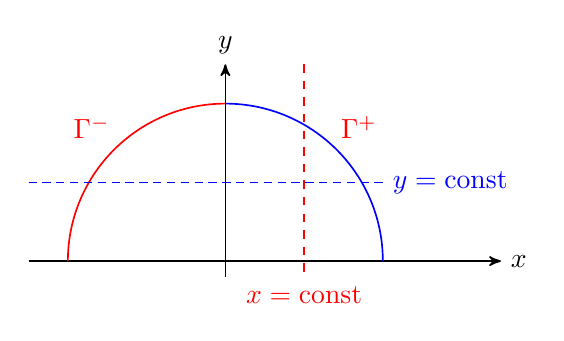
\begin{tikzpicture}[ media/.style={font={\footnotesize\sffamily}},
    interface/.style={
        postaction={draw,decorate,decoration={border,angle=-45,
                    amplitude=0.3cm,segment length=2mm}}},scale=2]

%\clip(-2,-2.4)rectangle(2.4,2.1);
\draw[semithick,->,>=stealth'](-1.25,0)--(1.75,0) node[right]{$x$};
\draw[semithick,->,>=stealth'](0,-0.1)--(0,1.25) node[above]{$y$};




\draw[semithick,red](-1,0) arc(180:90:1);
\node[red,semithick] at (135:1.2){$\Gamma^-$};
\draw[semithick,blue](1,0) arc(0:90:1);
\node[red,semithick] at (45:1.2){$\Gamma^+$};
\draw[blue,densely dashed,semithick] (-1.25,0.5)--(1,0.5) node[right]{$y=\textrm{const}$};

\draw[red,dashed,semithick] (0.5,1.25)--(0.5,-0.1) node[below]{$x=\textrm{const}$};


\end{tikzpicture}

\end{center}
\end{multicols}
\noindent 该解在与$x$轴平行的直线$y=\textrm{const}$上有相同的值, 因此不能满足$\Gamma^{+}$或$\Gamma^{-}$上的某一边界条件.
因此另一边界上出现边界层. 把原方程中的$y$看作参数, 并看作$x$为自变量的常微分方程, 由习题7.19知在$\Gamma^{+}$附近有边界层.
令
\[
\eta=\frac{x-x^{+}(y)}{\varepsilon}
\]
\[
u(x,y,\varepsilon)=V(\eta,y,\varepsilon)=V_{0}(\eta,y)+\cdots
\]
代入到原方程, 注意到
\[
\begin{array}{ll}
\displaystyle u_{x}=\frac{V_{\eta}}{\varepsilon}, & \displaystyle u_{xx}=\frac{V_{\eta\eta}}{\varepsilon^{2}}\\
\displaystyle u_{y}=V_{\eta}\frac{-{x'}^{+}(y)}{\varepsilon}+V_{y}, & \displaystyle u_{yy}=V_{\eta\eta}\Big[\frac{{x'}^{+}(y)}{\varepsilon}\Big]^{2}-V_{\eta}\frac{{x''}^{+}(y)}{\varepsilon}+2V_{y\eta}\frac{{x'}^{+}(y)}{\varepsilon}+V_{yy}
\end{array}
\]
可得
\begin{equation}
(1+[{x'}^{+}(y)]^{2})V_{\eta\eta}-V_{\eta}=0\label{eq:72901}
\end{equation}
其边界条件为
\[
V(0,y)=f^{+},V(-\infty,y)=f^{-}
\]
令$1+[{x'}^{+}(y)]^{2}=K$, 则方程(\ref{eq:72901})符合上述边界条件的解为
\[
V_{0}=(f^{+}-f^{-})e^{\eta/K}+f^{-}
\]


\vspace{1em}

\noindent 同样, 在与$y$轴平行的直线$x=\textrm{const}$上有相同的值, 因此不能满足$\Gamma$或$F$上的某一边界条件.
因此$F$上也出现边界层, 取内变量
\[
\xi=\frac{y}{\varepsilon^{\lambda}}, ~~ u(x,y,\varepsilon)=u(x,\xi,\varepsilon)=W(x,\xi)+\cdots
\]
代入到原方程, 注意到
\[
\begin{array}{ll}
\displaystyle u_{x}=W_{x}, & \displaystyle u_{xx}=W_{xx}\\
 &  \\
\displaystyle u_{y}=\frac{W_{\xi}}{\varepsilon^{\lambda}}, & \displaystyle u_{yy}=\frac{W_{\xi\xi}}{\varepsilon^{2\lambda}}
\end{array}
\]
可得
\[
\varepsilon\Big(\frac{W_{\xi\xi}}{\varepsilon^{2\lambda}}+W_{xx}\Big)=W_{x}
\]
为使$W_{\xi\xi}$与$W_{x}$同阶, $\lambda=1/2$. 因此上式变为
\[
W_{\xi\xi}-W_{x}=0
\]
其边界条件为
\[
W(x,0)=F(x), ~~ W(x,+\infty)=f(x), ~~ W(-R,0)=F(-R)=f(-R)
\]
符合上述边界条件$y=0$附近的内解为
\[
W_{0}=f(-R)+\int_{0}^{x+R}\frac{[F(\zeta)-f(-R)]\xi}{2\sqrt{\pi(x+R-\zeta)^{3}}}\exp\Big[\frac{-\xi^{2}}{4(x+R-\zeta)}\Big]d\zeta
\]

\end{solution}



\newpage
\appendix
\appendixpage
\lhead{附录: 试题}
\invisiblesection{摄动理论2012年期末试题}
\problemlist{\bf 摄动理论2012年期末试题\footnote{{\bf 说明:} 本试题是本人考试后立刻回忆出来的, 供后届同学参考.}}

\begin{enumerate}
\item 确定下列函数的阶, 并按大小排列($\varepsilon\rightarrow 0$)
\[
\ln\sinh\frac{1}{\varepsilon},\quad
\ln\csc\varepsilon,\quad
\exp\Big(\frac{\sqrt{1-\cos^2\varepsilon}}{-\sin\varepsilon^2}\Big),\:
\frac{1-\cos\varepsilon}{\varepsilon^{4/3}},\quad
\tan\sqrt{\varepsilon},\quad
\ln(2+\sin\varepsilon),\quad
\]
\[
\varepsilon\sin\varepsilon,\quad
\ln\bigg[1+\frac{\ln(1+1\varepsilon)}{1-\varepsilon}\bigg],\quad
\varepsilon^{1/2}(1-\cos\varepsilon)^{-1/2},\quad
\ln(1+\varepsilon)
\]

\vspace{0.5em}
\item 试求下述问题的首项解
\[
u''+\varepsilon u'+u +\varepsilon u^3 = 0
\]

\vspace{0.5em}
\item 试求下述问题的可解性条件.
\[
u'' + 4u= f(x),\:
u(0) = a, \:
u'(\pi/4)=b
\]

\vspace{0.5em}
\item 试求一致有效展开的首项
\[
\varepsilon y'' + xy' + xy = 0,\:
u(0)=\alpha,\:
y(1) = \beta
\]
\end{enumerate} 

\newpage
\invisiblesection{渐进分析2011年期末试题}
\problemlist{\bf 渐进分析2011年期末试题\footnote{{\bf 说明:} 2012年的试题与2011年试题相仿.}} 
\begin{center}
\fbox{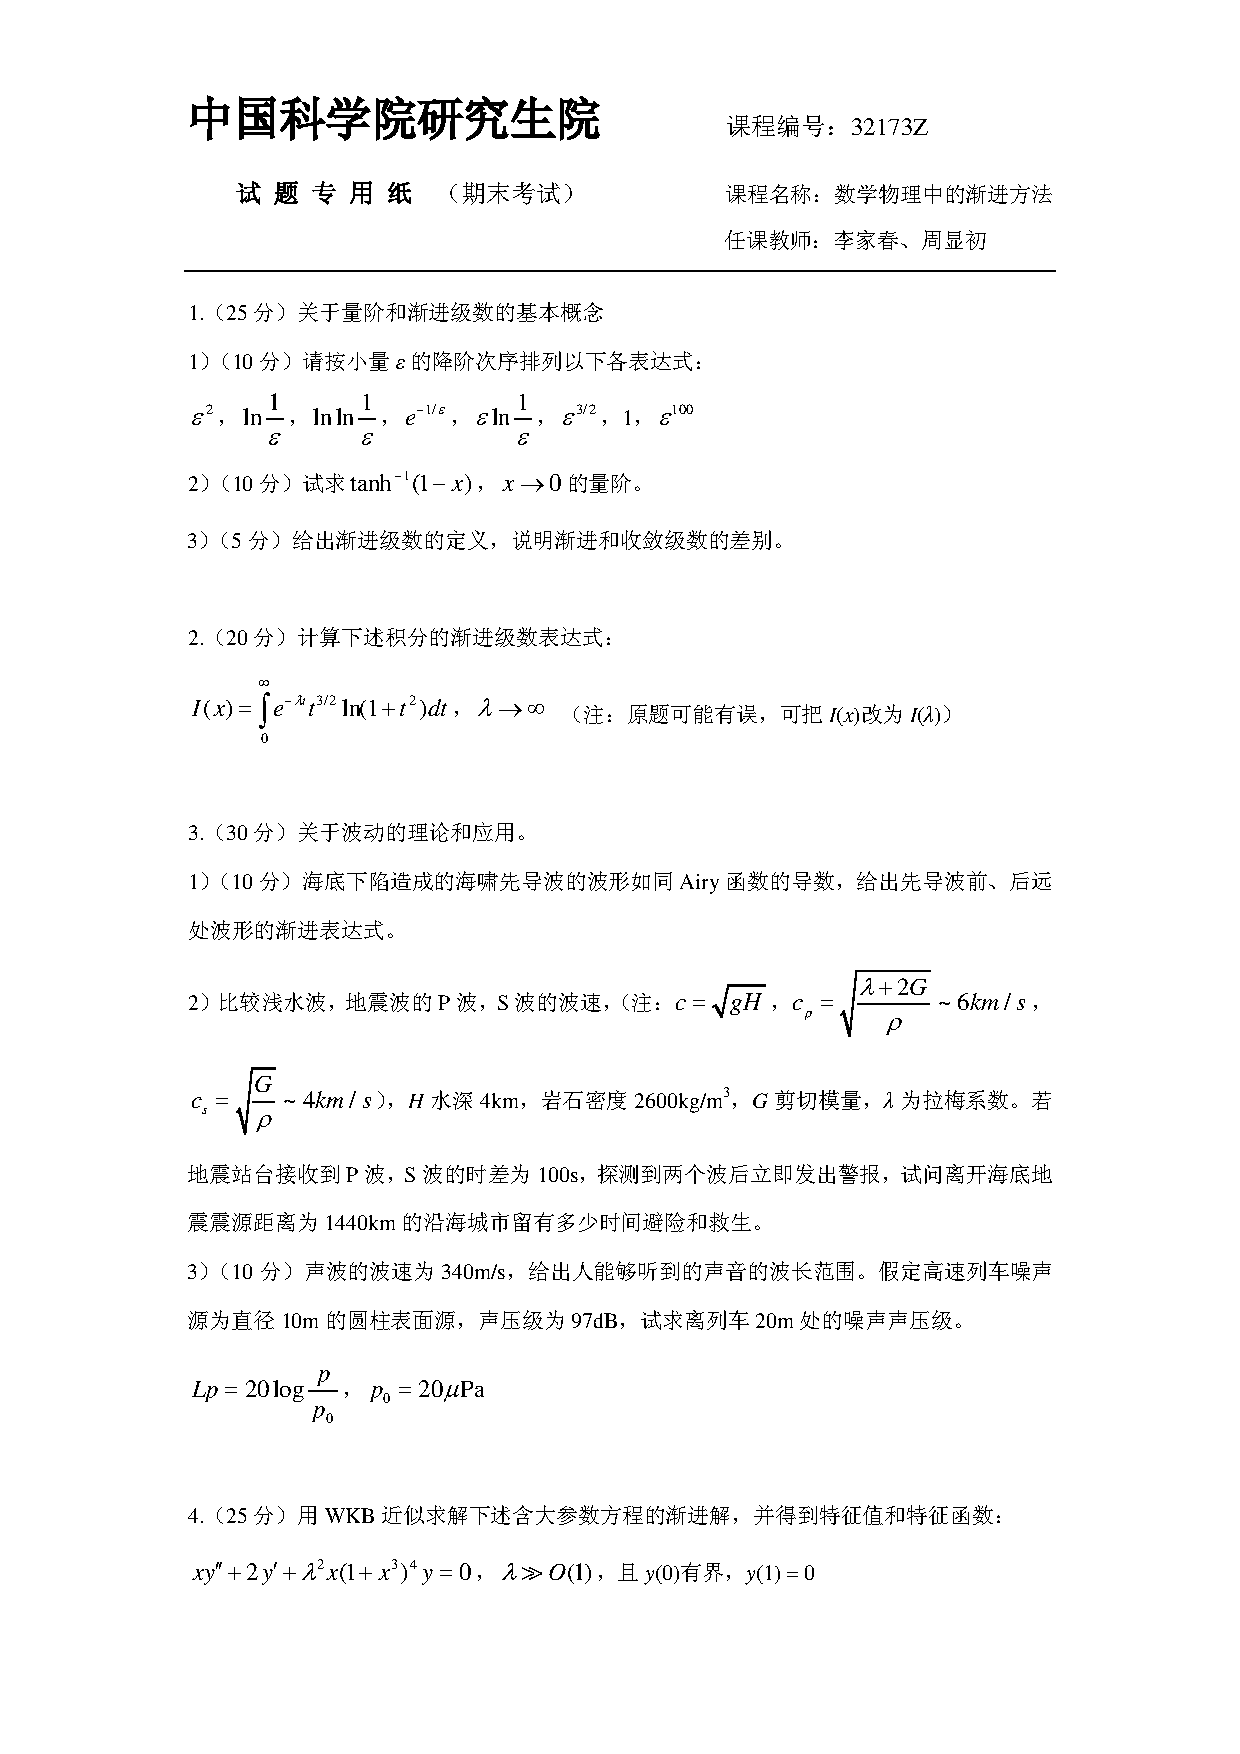
\includegraphics[width=0.95\textwidth]{exam2.pdf}}
\end{center}

\end{document} 
